\section{建模与求解}
这里将通过数学建模,讨论并解决本文所提出的2个问题。首先建立通用的几何体归类判别模型框架,然后分别应用于平面五边形和三维八面体的归类问题。共分为2个小节。

\subsection{问题一的建模与求解}
问题一主要解决平面五边形的归类判别问题。本节将详细阐述我们提出的基于多尺度特征与全局优化Kabsch配准的平面五边形判别模型。

该模型的核心思想是融合两种不同但互补的相似性度量:一是基于8维几何特征向量的相似性度量(特征距离$d_{\mathcal{F}}$),它从多个角度捕捉五边形的几何不变量特性;二是基于Kabsch全局优化算法的几何配准吻合度(均方根误差$RMSD$),它直接量化两个五边形点集在最优空间对齐下的几何差异。通过引入权重参数$\alpha_p$将这两种度量组合为一个综合评分$S$,并结合优化确定的分类阈值$\lambda_p$,实现对观测五边形的精确归类。

本小节主要内容包括:五边形数据的预处理、基于多尺度特征与Kabsch配准的模型建立、模型的求解和分析、模型性能验证。

\subsubsection{数据的预处理} % 与图片一致的层级
\textbf{1. 数据采集与整理}

根据问题描述,我们整理了两类标准五边形和五个待测五边形的顶点坐标数据。标准类别I和类别II的五边形顶点坐标如表\ref{tab:std_polygons_bordered}所示,待测五边形的顶点坐标如表\ref{tab:test_polygons}所示。


\begin{table}[H] % 使用 [H] 来固定位置
\centering
\caption{标准类别I和类别II的五边形顶点坐标} % 添加标题
\label{tab:std_polygons_bordered} % 在caption之后添加标签
\begin{tabular}{|>{\centering\hspace{0pt}}m{0.133\linewidth}|>{\centering\hspace{0pt}}m{0.158\linewidth}|>{\centering\hspace{0pt}}m{0.158\linewidth}|>{\centering\hspace{0pt}}m{0.158\linewidth}|>{\centering\hspace{0pt}}m{0.158\linewidth}|>{\centering\arraybackslash\hspace{0pt}}m{0.167\linewidth}|}
\hline
类别 & 顶点一         & 顶点二         & 顶点三         & 顶点四         & 顶点五          \\
\hline
I  & (0.74,1.90) & (1.26,3.49) & (3.54,3.58) & (3.13,2.28) & (4.45,1.16)  \\
\hline
II & (0.71,2.75) & (1.65,4.08) & (2.58,3.09) & (1.31,2.66) & (1.13,1.75)  \\
\hline
\end{tabular}
\end{table}

\begin{table}[H] % 使用 [H] 来固定位置
\centering
\caption{待测五边形的顶点坐标} % 添加标题
\label{tab:test_polygons} % 在caption之后添加标签
\begin{tabular}{|>{\centering\hspace{0pt}}m{0.133\linewidth}|>{\centering\hspace{0pt}}m{0.158\linewidth}|>{\centering\hspace{0pt}}m{0.158\linewidth}|>{\centering\hspace{0pt}}m{0.158\linewidth}|>{\centering\hspace{0pt}}m{0.158\linewidth}|>{\centering\arraybackslash\hspace{0pt}}m{0.158\linewidth}|}
\hline
图形编号 & 顶点一         & 顶点二         & 顶点三         & 顶点四         & 顶点五          \\
\hline
1    & (5.69,3.94) & (5.62,4.31) & (6.07,4.61) & (6.13,4.29) & (6.53,4.21)  \\
\hline
2    & (1.14,2.07) & (2.55,3.24) & (5.07,2.04) & (5.03,4.78) & (1.88,4.11)  \\
\hline
3    & (1.80,2.76) & (4.08,3.04) & (2.26,3.25) & (1.96,4.54) & (1.19,3.61)  \\
\hline
4    & (5.74,2.94) & (3.96,3.38) & (3.69,4.78) & (1.68,3.49) & (1.98,1.86)  \\
\hline
5    & (1.60,4.79) & (2.46,1.93) & (5.26,3.42) & (5.31,5.80) & (4.40,4.25)  \\
\hline
\end{tabular}
\end{table}
    \textbf{2. 顶点归一化处理}
    
    为了消除平移、旋转和尺度差异的影响,我们需要对五边形进行归一化处理。归一化步骤如下:
    \textbf{(1)} 计算五边形的重心 $\mathbf{c} = \frac{1}{n}\sum_{i=1}^{n}\mathbf{p}_i$,其中 $n=5$ 为顶点数量。
    \textbf{(2)} 将重心平移到原点:$\mathbf{p}'_i = \mathbf{p}_i - \mathbf{c}$。
    \textbf{(3)} 计算最大边长 $L = \max_{i,j} \|\mathbf{p}'_i - \mathbf{p}'_j\|$。
    \textbf{(4)} 按最大边长归一化坐标:$\mathbf{p}''_i = \mathbf{p}'_i / L$。

图\ref{fig:normalize}展示了一个五边形归一化处理前后的对比。通过归一化,我们可以消除几何体间的位置、方向和大小差异,使后续的特征提取和配准更加可靠。

\begin{figure}[H] % [H] 选项来自 float 宏包,表示将图片"确实放在这里"
    \centering      % 图片居中显示
    % 在此处插入五边形归一化过程的图示
    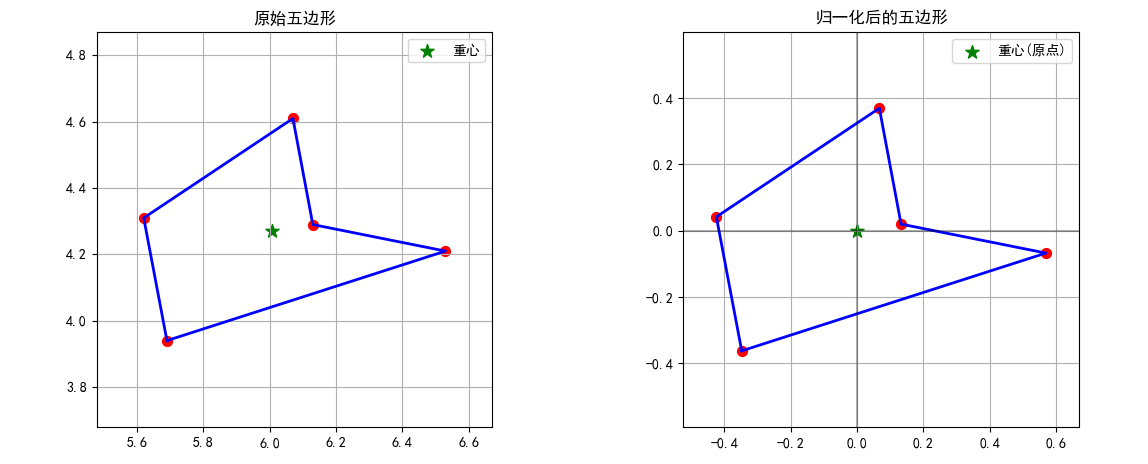
\includegraphics[width=1\textwidth]{figures/pentagon_normalization.png}
    % 注意路径修改为 "figures/pentagon_normalization.png"
    %
    % 说明:
    % 1. figures/pentagon_normalization.png 是您的图片文件相对于 .tex 文件的路径。
    % 2. [width=0.8\textwidth] 是一个可选参数,用于设置图片的宽度。
    %    0.8\textwidth 表示图片宽度为当前文本宽度的 80%。
    %    您可以根据需要调整这个值。
    \caption{五边形归一化处理示例}
    \label{fig:normalize} % \label 必须放在 \caption 之后或内部,以便正确引用
\end{figure}

\subsubsection{基于多尺度特征与刚性配准的五边形归类模型的建立}

\textbf{1. 模型总体框架与核心思想}

在完成五边形顶点坐标的中心化和尺度归一化预处理后,我们需要构建一个能够有效区分不同类别五边形的判别模型。本节将详细阐述我们提出的结合多尺度几何特征与Kabsch全局优化算法的平面五边形归类判别模型。

该模型的核心思想是融合两种不同但互补的相似性度量:一是基于8维几何特征向量的相似性度量(特征距离$d_{\mathcal{F}}$),它从多个角度捕捉五边形的几何不变量特性;二是基于Kabsch全局优化算法的几何配准吻合度(均方根误差$RMSD$),它直接量化两个五边形点集在最优空间对齐下的几何差异。通过引入权重参数$\alpha_p$将这两种度量组合为一个综合评分$S$,并结合优化确定的分类阈值$\lambda_p$,实现对观测五边形的精确归类。

图\ref{fig:model_framework}展示了本模型的完整框架,从预处理后的五边形点集输入,经过特征提取和Kabsch配准两条并行路径,最终通过综合评分机制得出分类结果。该框架图直观地呈现了模型各组件间的信息流动和处理逻辑,突显了多尺度特征与几何配准的融合思想。

\begin{figure}[H]
    \centering
    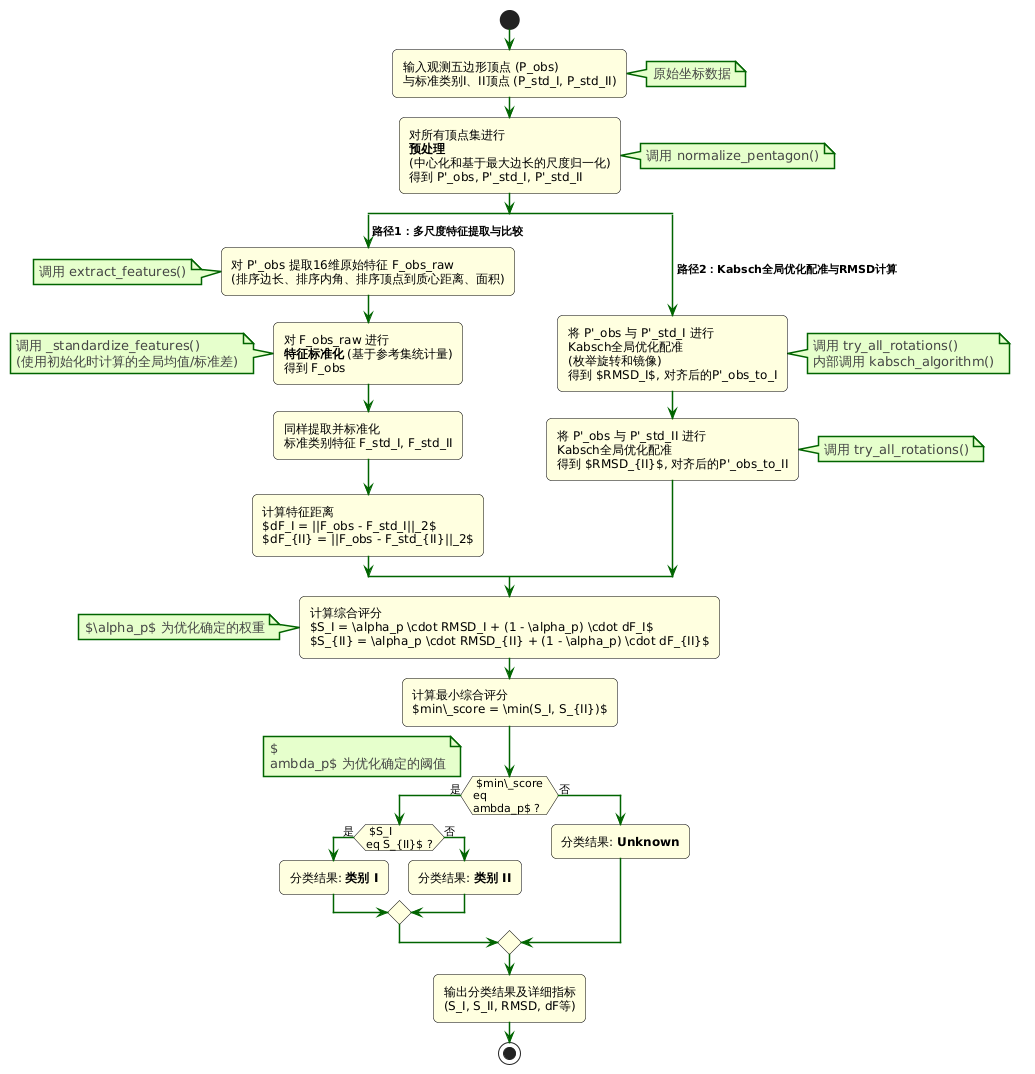
\includegraphics[width=1\textwidth]{figures/model1.png}
    \caption{基于多尺度特征与全局优化Kabsch配准的平面五边形判别模型的整体框架}
    \label{fig:model_framework}
\end{figure}

\textbf{2. 几何不变量特征提取与标准化}

对于归一化后的五边形,我们提取以下几何不变量特征:

\textbf{(1)} 边长序列:计算五边形各边长度,并按从小到大排序,形成边长序列向量。
\begin{equation}
    \mathbf{L} = [l_1, l_2, l_3, l_4, l_5]
\end{equation}
其中,$l_i = \|\mathbf{p}_i - \mathbf{p}_{i+1}\|$($i=1,2,3,4$),$l_5 = \|\mathbf{p}_5 - \mathbf{p}_1\|$。

\textbf{(2)} 内角序列:计算五边形各内角,并按从小到大排序,形成内角序列向量。
\begin{equation}
   \bm{\Theta} = [\theta_1, \theta_2, \theta_3, \theta_4, \theta_5]
\end{equation}
其中,$\theta_i$为第$i$个顶点处的内角。

\textbf{(3)} 顶点到质心的距离序列:计算各顶点到质心的距离,并按从小到大排序。
\begin{equation}
    \mathbf{D} = [d_1, d_2, d_3, d_4, d_5]
\end{equation}
其中,$d_i = \|\mathbf{p}_i - \mathbf{c}\|$为第$i$个顶点到质心的欧氏距离。

\textbf{(4)} 面积:计算五边形的面积。
\begin{equation}
    A = \frac{1}{2}\left|\sum_{i=1}^{5} x_i(y_{i+1} - y_{i-1})\right|
\end{equation}
其中,$x_i$和$y_i$是顶点$i$的坐标,下标使用循环索引。

最终,我们构建特征向量$\mathcal{F} = [\mathbf{L}, \bm{\Theta}, \mathbf{D}, A]$。

为了解决不同类型特征之间的量纲差异问题并优化特征空间分布,我们对提取的原始特征向量进行Z-score标准化处理:
\begin{equation}
    \mathcal{F}_{\text{normalized}} = \frac{\mathcal{F} - \mu_{\mathcal{F}}}{\sigma_{\mathcal{F}}}
\end{equation}
其中$\mu_{\mathcal{F}}$和$\sigma_{\mathcal{F}}$分别是基于参考形状集(包括标准类别和负样本)计算的特征均值和标准差向量。特征标准化确保了不同特征维度在计算特征距离时具有可比性,避免了某些具有较大绝对值的特征(如面积)对分类决策产生过度影响。

\textbf{3. Kabsch刚性配准算法}

对于两个点集$P = \{\mathbf{p}_1, \mathbf{p}_2, ..., \mathbf{p}_n\}$和$Q = \{\mathbf{q}_1, \mathbf{q}_2, ..., \mathbf{q}_n\}$,Kabsch算法\cite{kabsch1976solution}通过以下步骤找到最优刚性变换(旋转矩阵$\mathbf{R}$和平移向量$\mathbf{t}$),使得变换后的点集与目标点集之间的均方根距离(Root Mean Square Distance, RMSD)最小:

\textbf{(1)} 计算两个点集的重心(质心):
\begin{align}
    \mathbf{c}_P &= \frac{1}{n}\sum_{i=1}^{n}\mathbf{p}_i \\
    \mathbf{c}_Q &= \frac{1}{n}\sum_{i=1}^{n}\mathbf{q}_i
\end{align}
其中 $\mathbf{c}_P$ 和 $\mathbf{c}_Q$ 分别是点集 $P$ 和 $Q$ 的重心。

\textbf{(2)} 将点集去中心化(即将重心平移至原点):
\begin{align}
    \mathbf{p}'_i &= \mathbf{p}_i - \mathbf{c}_P \\
    \mathbf{q}'_i &= \mathbf{q}_i - \mathbf{c}_Q
\end{align}
得到新的点集 $P' = \{\mathbf{p}'_1, ..., \mathbf{p}'_n\}$ 和 $Q' = \{\mathbf{q}'_1, ..., \mathbf{q}'_n\}$。

\textbf{(3)} 计算协方差矩阵(或称为交叉协方差矩阵)$\mathbf{H}$:
\begin{equation}
    \mathbf{H} = \sum_{i=1}^{n}\mathbf{p}'_i {\mathbf{q}'_i}^T
\end{equation}
这里假设 $\mathbf{p}'_i$ 和 $\mathbf{q}'_i$ 是列向量。因此,$\mathbf{p}'_i {\mathbf{q}'_i}^T$ 是一个 $d \times d$ 的矩阵(其中 $d$ 是点的维度,例如平面点为2,空间点为3),$\mathbf{H}$ 是这些矩阵的和。

\textbf{(4)} 对协方差矩阵 $\mathbf{H}$ 进行奇异值分解(SVD):
\begin{equation}
    \mathbf{H} = \mathbf{U}\bm{\Sigma} \mathbf{V}^T
\end{equation}
其中:
\begin{itemize}
    \item $\mathbf{U}$ 是一个 $d \times d$ 的正交矩阵,其列是 $\mathbf{H}\mathbf{H}^T$ 的特征向量(左奇异向量)。
    \item $\bm{\Sigma}$ 是一个 $d \times d$ 的对角矩阵,对角线上的元素 $\sigma_j$ 是 $\mathbf{H}$ 的奇异值,它们是非负的并按降序排列。
    \item $\mathbf{V}$ 是一个 $d \times d$ 的正交矩阵,其列是 $\mathbf{H}^T\mathbf{H}$ 的特征向量(右奇异向量)。$\mathbf{V}^T$ 是 $\mathbf{V}$ 的转置。
\end{itemize}

\textbf{(5)} 计算最优旋转矩阵 $\mathbf{R}$:
\begin{equation}
    \mathbf{R} = \mathbf{V} \mathbf{U}^T
\end{equation}
为了确保 $\mathbf{R}$ 是一个纯旋转矩阵(即 $\det(\mathbf{R}) = 1$)而不是一个包含反射的变换(即 $\det(\mathbf{R}) = -1$),需要检查其行列式。如果 $\det(\mathbf{R}) = -1$,则需要进行修正。一个标准的修正是:
令 $\mathbf{S} = \mathrm{diag}(1, \dots, 1, \det(\mathbf{V}\mathbf{U}^T))$。如果 $\det(\mathbf{V}\mathbf{U}^T) = -1$,则 $\mathbf{S}$ 的最后一个对角元素为 $-1$。
最优的旋转矩阵则为 $\mathbf{R} = \mathbf{V} \mathbf{S} \mathbf{U}^T$。
在实践中,如果 $\det(\mathbf{V}\mathbf{U}^T) = -1$,通常是将 $\mathbf{V}$ 的最后一列(或者 $\mathbf{U}$ 的最后一列,取决于约定)乘以 $-1$ 得到 $\mathbf{V}'$ (或 $\mathbf{U}'$),然后重新计算 $\mathbf{R} = \mathbf{V}' \mathbf{U}^T$ (或 $\mathbf{R} = \mathbf{V} (\mathbf{U}')^T$)。例如,若取 $\mathbf{V}'$ 的最后一列为 $\mathbf{V}$ 最后一列的相反数,则 $\mathbf{R} = \mathbf{V}' \mathbf{U}^T$。

\textbf{(6)} 计算最优平移向量 $\mathbf{t}$:
\begin{equation}
    \mathbf{t} = \mathbf{c}_Q - \mathbf{R}\mathbf{c}_P
\end{equation}
最终,点集 $P$ 中的任意点 $\mathbf{p}$ 可以通过 $\mathbf{p}_{transformed} = \mathbf{R}\mathbf{p} + \mathbf{t}$ 变换到尽量接近点集 $Q$ 中对应点的位置。
    
    \textbf{4. 考虑所有可能的旋转排列}
    
    由于五边形的顶点排序可能会影响配准结果,我们引入了一种尝试所有可能旋转排序的策略:
    
    \textbf{(1)} 对于五边形的五个顶点,我们尝试所有可能的起始顶点(5种排序)。
    
    \textbf{(2)} 对于每种排序,我们还考虑顺时针和逆时针两种方向(相当于10种不同排序)。
    
    \textbf{(3)} 对每种排序方式应用Kabsch算法,计算RMSD。
    
    \textbf{(4)} 选择产生最小RMSD的排序作为最终结果。
    
    \textbf{5. 综合评估与归类判别模型}
    
    对于待归类的五边形$X$,我们分别与标准类别$I$和$II$计算以下指标:
    
    \textbf{(1)} 特征相似度:计算标准化特征向量之间的欧氏距离,
    \begin{align}
        d_{\mathcal{F},I} &= \|\mathcal{F}_{X,\text{normalized}} - \mathcal{F}_{I,\text{normalized}}\| \\
        d_{\mathcal{F},II} &= \|\mathcal{F}_{X,\text{normalized}} - \mathcal{F}_{II,\text{normalized}}\|
    \end{align}
    
    (2) 配准误差:使用优化的Kabsch算法将$X$与$I$、$II$分别进行配准,计算均方根误差(RMSD),
    \begin{align}
        RMSD_I &= \sqrt{\frac{1}{n}\sum_{i=1}^{n}\|\mathbf{p}^X_i - \mathbf{p}^I_i\|^2} \\
        RMSD_{II} &= \sqrt{\frac{1}{n}\sum_{i=1}^{n}\|\mathbf{p}^X_i - \mathbf{p}^{II}_i\|^2}
    \end{align}
    
    (3) 综合评分:结合特征相似度和配准误差,计算综合评分,
\begin{align}
        S_I &= \alpha \cdot RMSD_I + (1-\alpha) \cdot d_{\mathcal{F},I} \\
        S_{II} &= \alpha \cdot RMSD_{II} + (1-\alpha) \cdot d_{\mathcal{F},II}
\end{align}
    其中$\alpha$为权重参数,通过参数优化确定。特征标准化确保了RMSD和特征距离在相似的数值范围内,使它们在综合评分中具有合理的相对贡献。
    
    (4) 归类判别:
    \begin{equation}
        \text{类别}(X) = 
        \begin{cases}
            I, & \text{if } S_I < S_{II} \text{ and } S_I < \lambda \\
            II, & \text{if } S_{II} < S_{I} \text{ and } S_{II} < \lambda \\
            \text{未知类别}, & \text{otherwise}
        \end{cases}
    \end{equation}
    其中$\lambda$为阈值参数,通过参数优化确定。
    

\subsubsection{模型的求解和分析}
    \textbf{1. 计算方法和算法实现}
    
  我们使用Python实现了基于多尺度特征与刚性配准的平面五边形归类判别模型。算法实现包含以下主要步骤:

\begin{algorithm}[H] % [H] 选项来自 float 宏包
\caption{五边形归类判别算法}
\label{alg:polygon_classification}
\begin{algorithmic}[1] % [1] 表示显示行号
    \Function{ClassifyPolygon}{$P, \mathit{ClassI}, \mathit{ClassII}$}
        \State 对输入的待测五边形$P$、类别I模板$\mathit{ClassI}$、类别II模板$\mathit{ClassII}$进行归一化处理
        \State 提取$P$的几何不变量特征向量$\mathcal{F}_P$
        \State 提取$\mathit{ClassI}$的几何不变量特征向量$\mathcal{F}_I$
        \State 提取$\mathit{ClassII}$的几何不变量特征向量$\mathcal{F}_{II}$
        \State 计算$P$与$\mathit{ClassI}$的特征向量欧氏距离 $d_{\mathcal{F},I} = \|\mathcal{F}_P - \mathcal{F}_I\|_2$
        \State 计算$P$与$\mathit{ClassII}$的特征向量欧氏距离 $d_{\mathcal{F},II} = \|\mathcal{F}_P - \mathcal{F}_{II}\|_2$
        \State 尝试所有可能的顶点对应和旋转,使用Kabsch算法计算$P$与$\mathit{ClassI}$和$\mathit{ClassII}$之间的最优刚性配准,得到$\mathit{RMSD}_{I}$和$\mathit{RMSD}_{II}$
        \State 计算$P$与$\mathit{ClassI}$的综合相似度评分 $S_I = \alpha \cdot \mathit{RMSD}_I + (1-\alpha) \cdot d_{\mathcal{F},I}$ 
        \State 计算$P$与$\mathit{ClassII}$的综合相似度评分 $S_{II} = \alpha \cdot \mathit{RMSD}_{II} + (1-\alpha) \cdot d_{\mathcal{F},II}$
        \If{$S_I < S_{II}$ \textbf{and} $S_I < \lambda$} \Comment{$\lambda$为预设阈值}
            \State \Return 类别I
        \ElsIf{$S_{II} < S_I$ \textbf{and} $S_{II} < \lambda$}
            \State \Return 类别II
        \Else
            \State \Return 未知类别
        \EndIf
    \EndFunction
\end{algorithmic}
\end{algorithm}

\textbf{2. 参数优化与敏感性分析}\

为确保模型的最佳性能,我们对分类器中的两个关键超参数进行了系统性的寻优:其一是综合评分中形状配准度量(RMSD)的权重$\alpha$,它平衡了几何刚性匹配程度与特征向量相似度的相对贡献;其二是归类阈值$\lambda$,它决定了将一个未知五边形判定为某个特定类别或"未知类别"的判别边界。这两个参数的精确选择对模型的识别准确率、类别区分能力以及对噪声和形变的鲁棒性至关重要。

我们采用网格搜索方法,在参数空间$\alpha \in [0, 1]$(步长0.05)和$\lambda \in [0, 1]$(步长0.05)中系统性地评估每一个参数组合的性能。评估目标是找到能够最大化综合评估函数的参数组合,该评估函数考虑了:

\begin{itemize}
    \item 对标准类别样本的正确识别率
    \item 对负样本(不属于任何已知类别的五边形)的正确拒绝率
    \item 不同类型错误判断的惩罚权重(例如,将负样本错误判为已知类别的惩罚大于将其中一个类别错判为另一个类别)
\end{itemize}

图\ref{fig:pentagon_params_heatmap}展示了参数优化的结果。从图中可以清晰地观察到在参数空间中存在一个高性能区域(图中右上方红色区域),在该区域内模型表现最优。经过详细分析,确定了最优参数组合$\alpha$和$\lambda$。

\begin{figure}[H]
    \centering
    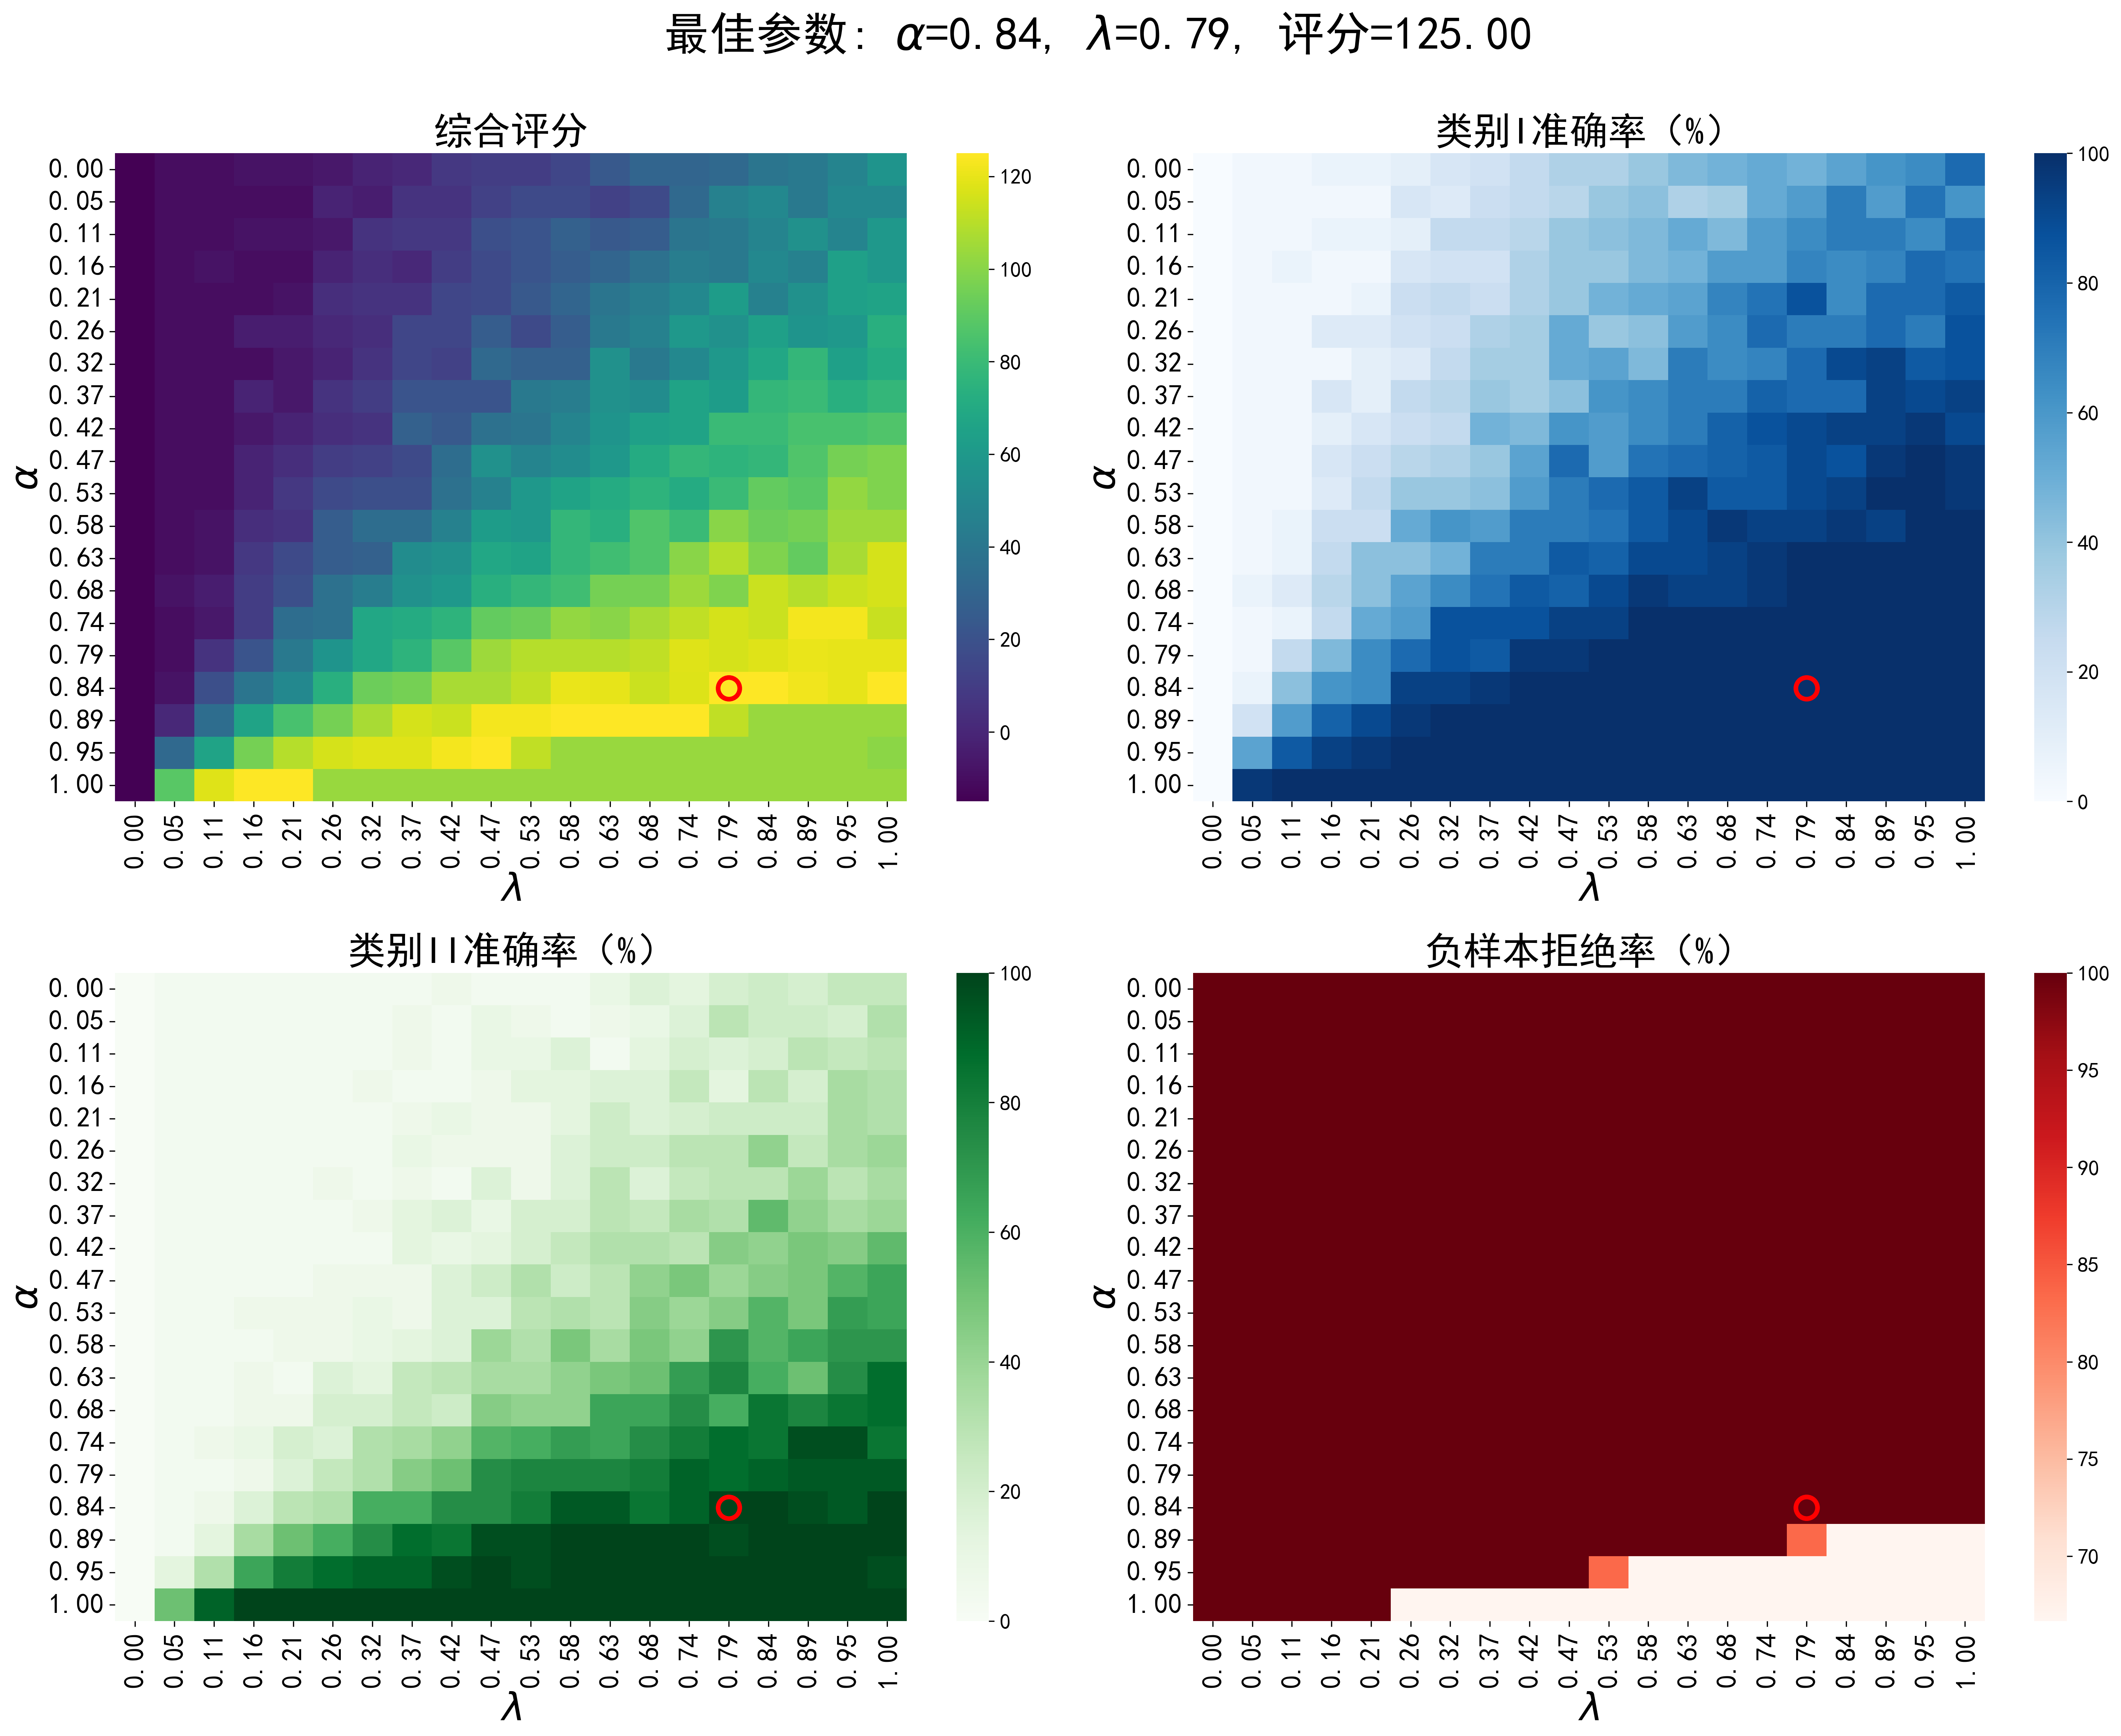
\includegraphics[width=0.9\textwidth]{../figures/params/pentagon_parameter_optimization_heatmaps.png}
    \caption{五边形归类模型参数优化热力图}
    \label{fig:pentagon_params_heatmap}
\end{figure}

图\ref{fig:param_optimization_3d1}以三维曲面图形式展示了相同的优化结果,提供了参数空间中模型性能变化的直观立体视图。从图中可见,参数性能曲面在最优参数$\alpha$和$\lambda$附近达到最高点,且该区域周围性能平稳,表明模型对参数微小变化具有一定稳健性。

\begin{figure}[H]
    \centering
    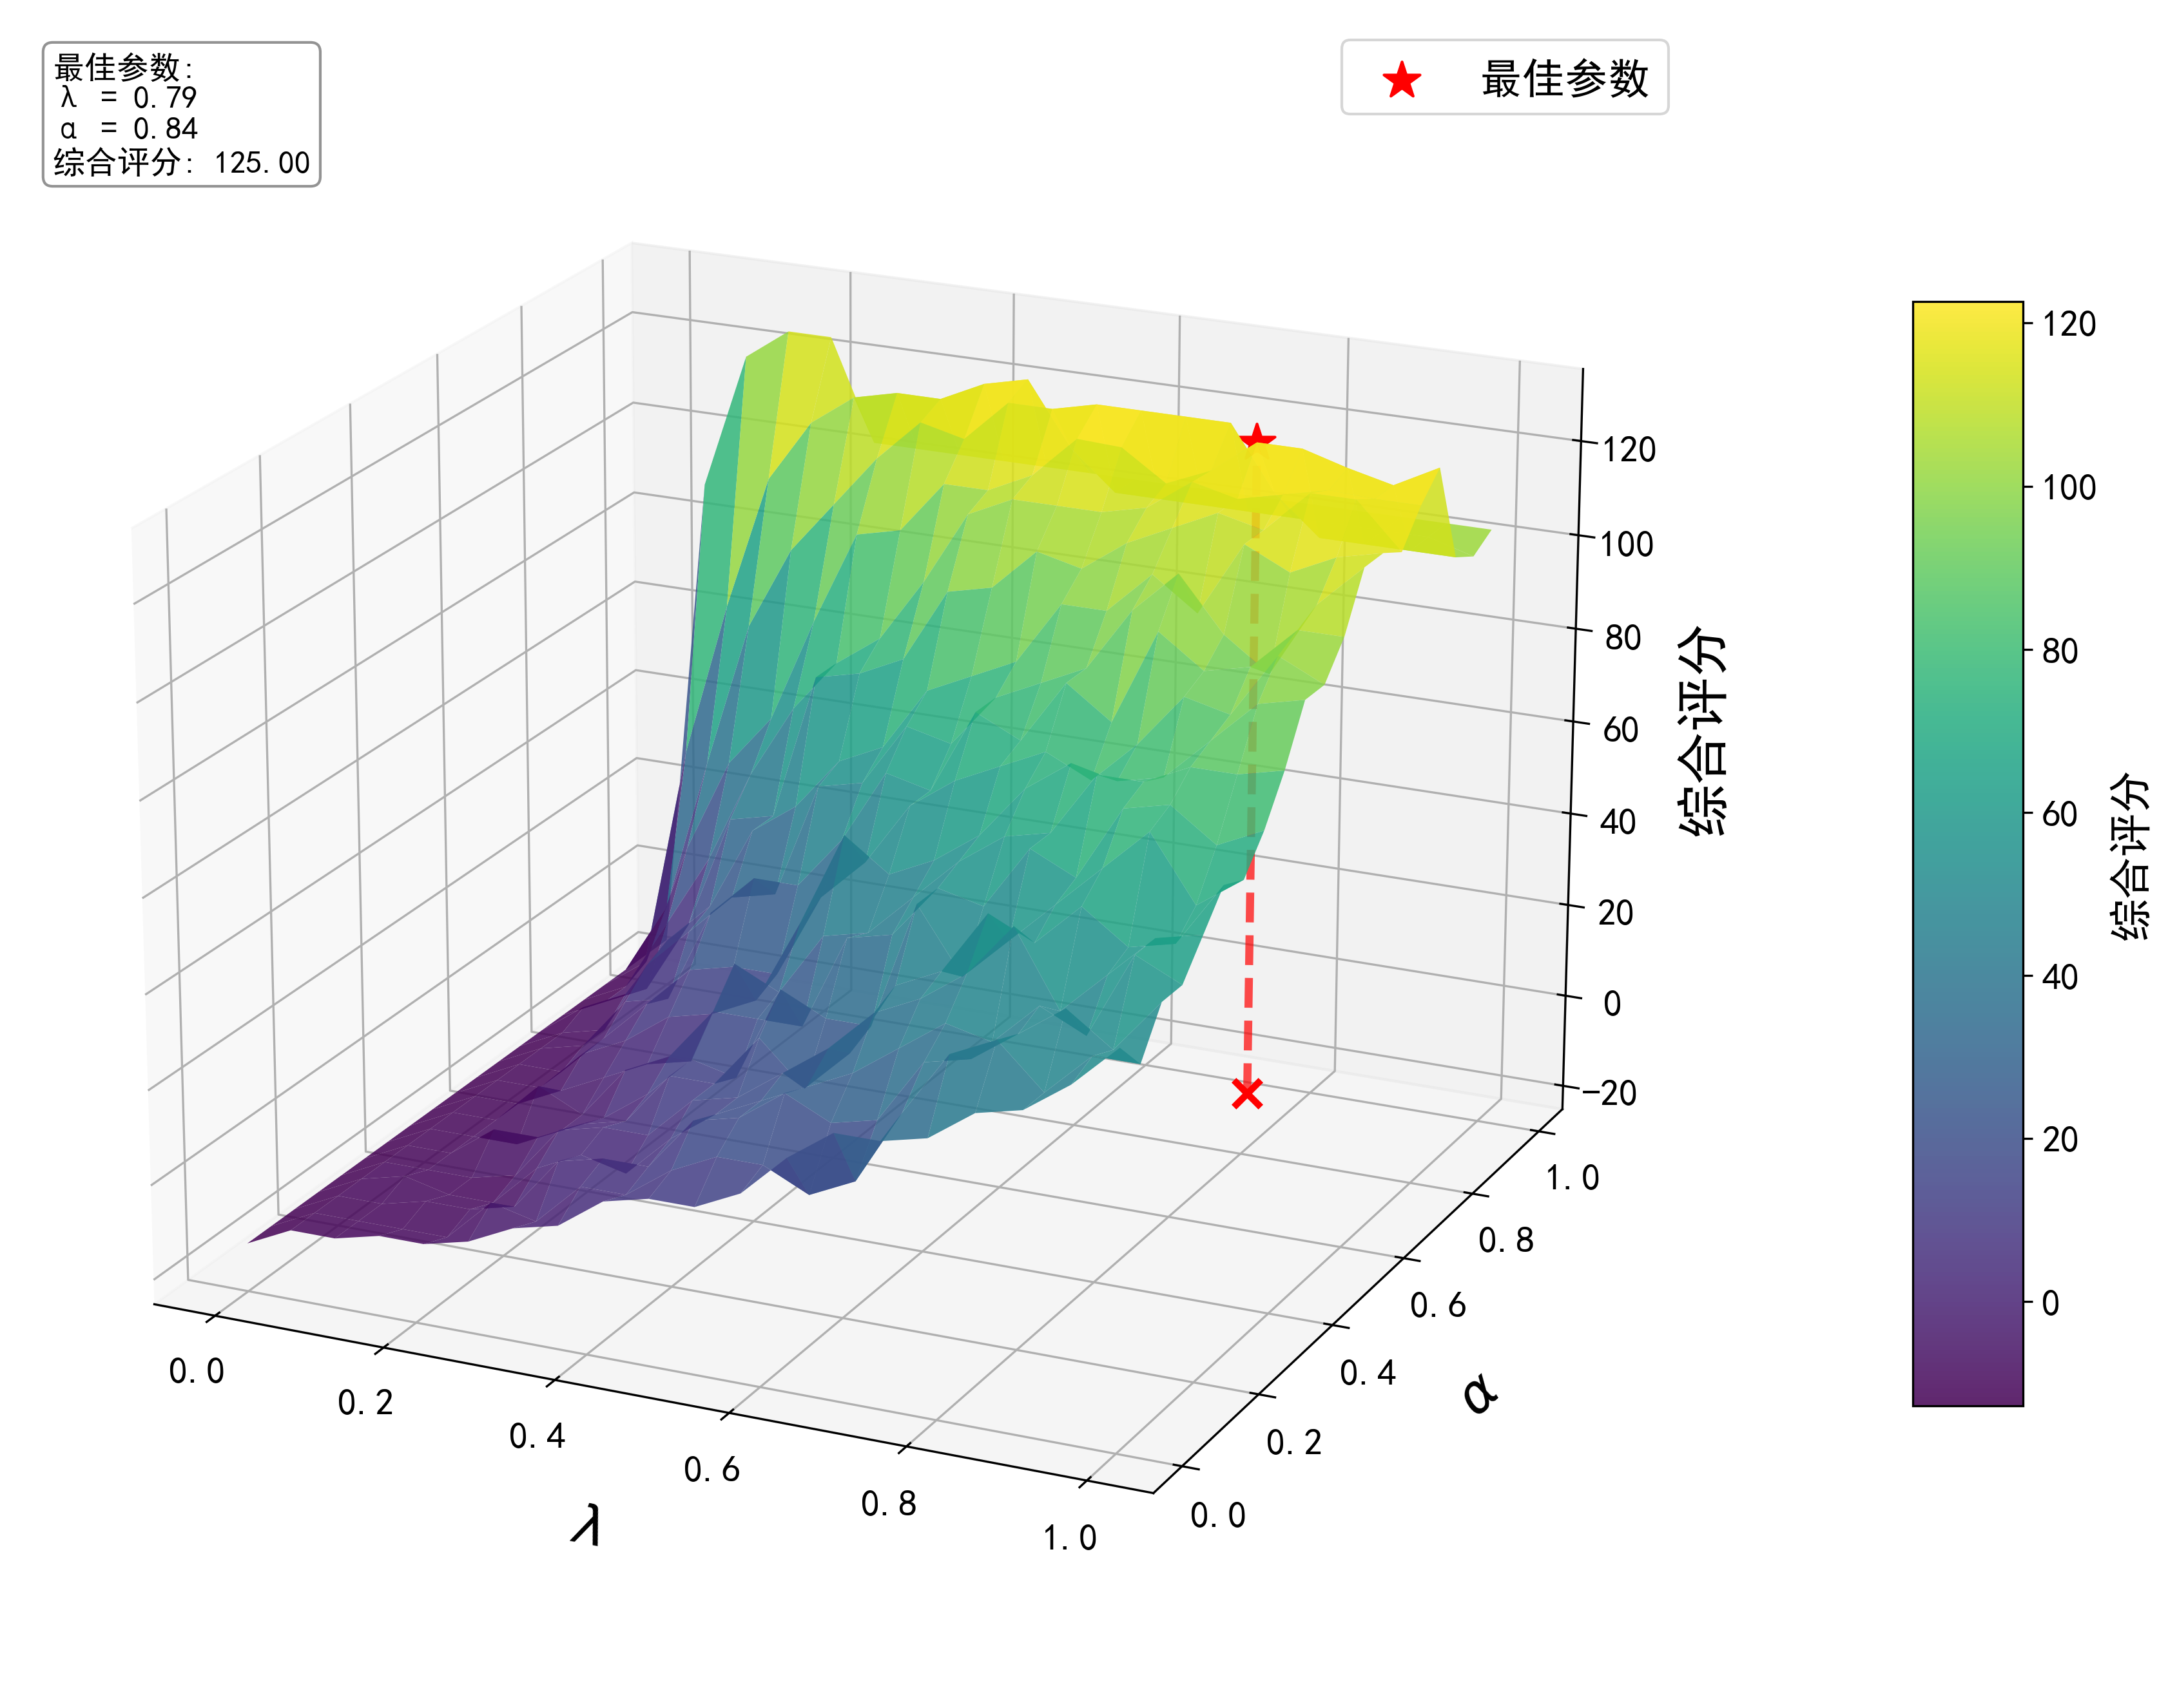
\includegraphics[width=0.8\textwidth]{figures/params/pentagon_parameter_optimization_3d.png}
    \caption{五边形分类模型参数优化结果三维曲面图}
    \label{fig:param_optimization_3d1}
\end{figure}

\phantomsection 
\textbf {注:关于评分模型量级差异说明} 值得注意的是,在参数优化评估函数中,我们为平面五边形问题设置了较高权重值(如正确识别的奖励权重为50.0,误判的惩罚权重为-40.0等),这导致评估函数的取值范围相对较大(如图\ref{fig:param_optimization_3d}所示,最优点处的综合评分约为125)。这种较大的权重设置主要基于以下考虑:一方面,平面五边形的参数空间结构特征较为复杂,需要更明确的梯度来引导优化过程;另一方面,为了在特征标准化后保持评估函数对边界情况(如接近判别阈值的样本)的敏感度。相比之下,三维八面体问题采用了较小的权重值(最优点综合评分约为44),这是由于其参数空间呈现更加平滑的响应曲面,无需过大的梯度驱动即可有效收敛。虽然两个问题的评估函数量级不同,但两者的相对权重比例(各类奖惩之间的相对关系)保持了概念上的一致性,确保了参数优化结果的可比性和合理性。此设计使得两个分类模型尽管在量级上有所差异,却能各自在其适用问题上达到最佳性能。
\label{bf:important_note}

\textbf{3. 计算结果与分析}
    
使用优化确定的参数$\alpha$和$\lambda$,我们对五个待测五边形进行了分类。表\ref{tab:results_q1}展示了详细的分类结果及关键指标。
    
   \begin{table}[H]
    \centering
    \caption{五边形归类结果}
    \label{tab:results_q1}
    \begin{tabular}{ccccccl}
    \toprule
    图形编号 & $RMSD_I$ & $RMSD_{II}$ & $d_{\mathcal{F},I}$ & $d_{\mathcal{F},II}$ & 综合评分(I/II) & 归类结果 \\
    \midrule
    1 & 0.0082 & 0.2956 & 0.3220 & 6.5186 & 0.0578 / 1.2782 & 类别I \\
    2 & 0.3010 & 0.0160 & 6.7958 & 0.4994 & 1.3265 / 0.0924 & 类别II \\
    3 & 0.1812 & 0.2235 & 4.4074 & 5.5873 & 0.8485 / 1.0704 & 未知类别 \\
    4 & 0.0101 & 0.2937 & 0.3142 & 6.5064 & 0.0581 / 1.2747 & 类别I \\
    5 & 0.3010 & 0.0489 & 7.8076 & 1.6174 & 1.4862 / 0.2965 & 类别II \\
    \bottomrule
    \end{tabular}
\end{table}

从表\ref{tab:results_q1}的数据分析可以得出以下结果:

\begin{enumerate}
    \item \textbf{图形1}的综合评分与类别I为0.0578,显著小于与类别II的评分1.2782,且远低于阈值$\lambda$,因此被明确判定为类别I。其极低的RMSD值(0.0082)和标准化特征距离(0.3220)共同表明它与标准类别I高度相似。

    \item \textbf{图形2}的综合评分与类别II为0.0924,远小于与类别I的评分1.3265,且低于阈值$\lambda$,因此被判定为类别II。其与类别II的低RMSD值(0.0160)表明在刚性配准上有极佳的匹配度。

    \item \textbf{图形3}的综合评分与类别I为0.8485,略高于阈值$\lambda$,与类别II的评分为1.0704,也高于阈值,因此被判定为未知类别。尽管其与类别I的相似度相对较高,但仍不足以达到归类标准。
    
    \item \textbf{图形4}的综合评分与类别I为0.0581,远小于与类别II的评分1.2747,且低于阈值$\lambda$,因此被判定为类别I。其低RMSD值(0.0101)和特征距离(0.3142)表明与类别I有高度匹配。
    
    \item \textbf{图形5}的综合评分与类别II为0.2965,明显小于与类别I的评分1.4862,且低于阈值$\lambda$,因此被判定为类别II。尽管其RMSD值(0.0489)略高于图形2,但仍然表明与类别II有良好的几何匹配。
\end{enumerate}

特征标准化的应用使得每个维度的特征对整体相似度的贡献更加平衡。从数据中可以观察到,特征距离值($d_{\mathcal{F},I}$和$d_{\mathcal{F},II}$)在不同类别间表现出明显的差异,这有助于提高分类决策的可靠性。特别是对于图形3,其RMSD值与其他样本相比并不特别高,但其特征距离值表明它与两个标准类别都存在一定差异,导致其综合评分超过了阈值,被正确判定为未知类别。

为更直观地展示各待测五边形的评分情况,图\ref{fig:pentagon_classification_scores}显示了五个观测五边形对两个标准模型的综合评分对比。从图中可以清晰看出,图形1和图形4与类别I的评分显著低于阈值线$\lambda$,而图形2和图形5与类别II的评分低于阈值线,符合我们的分类结果。图形3的综合评分无论是与类别I(0.8485)还是与类别II(1.0704)相比,都超过了阈值$\lambda$,因此被归类为未知类别。这一归类结果表明图形3与两个标准类别都存在一定差异,不足以被判定为任何已知类别。此图直观地展示了各五边形与两个标准类别的匹配程度差异,有助于理解分类决策的依据,特别是对于图形3这类边界情况的判定原理。

\begin{figure}[H]
    \centering
    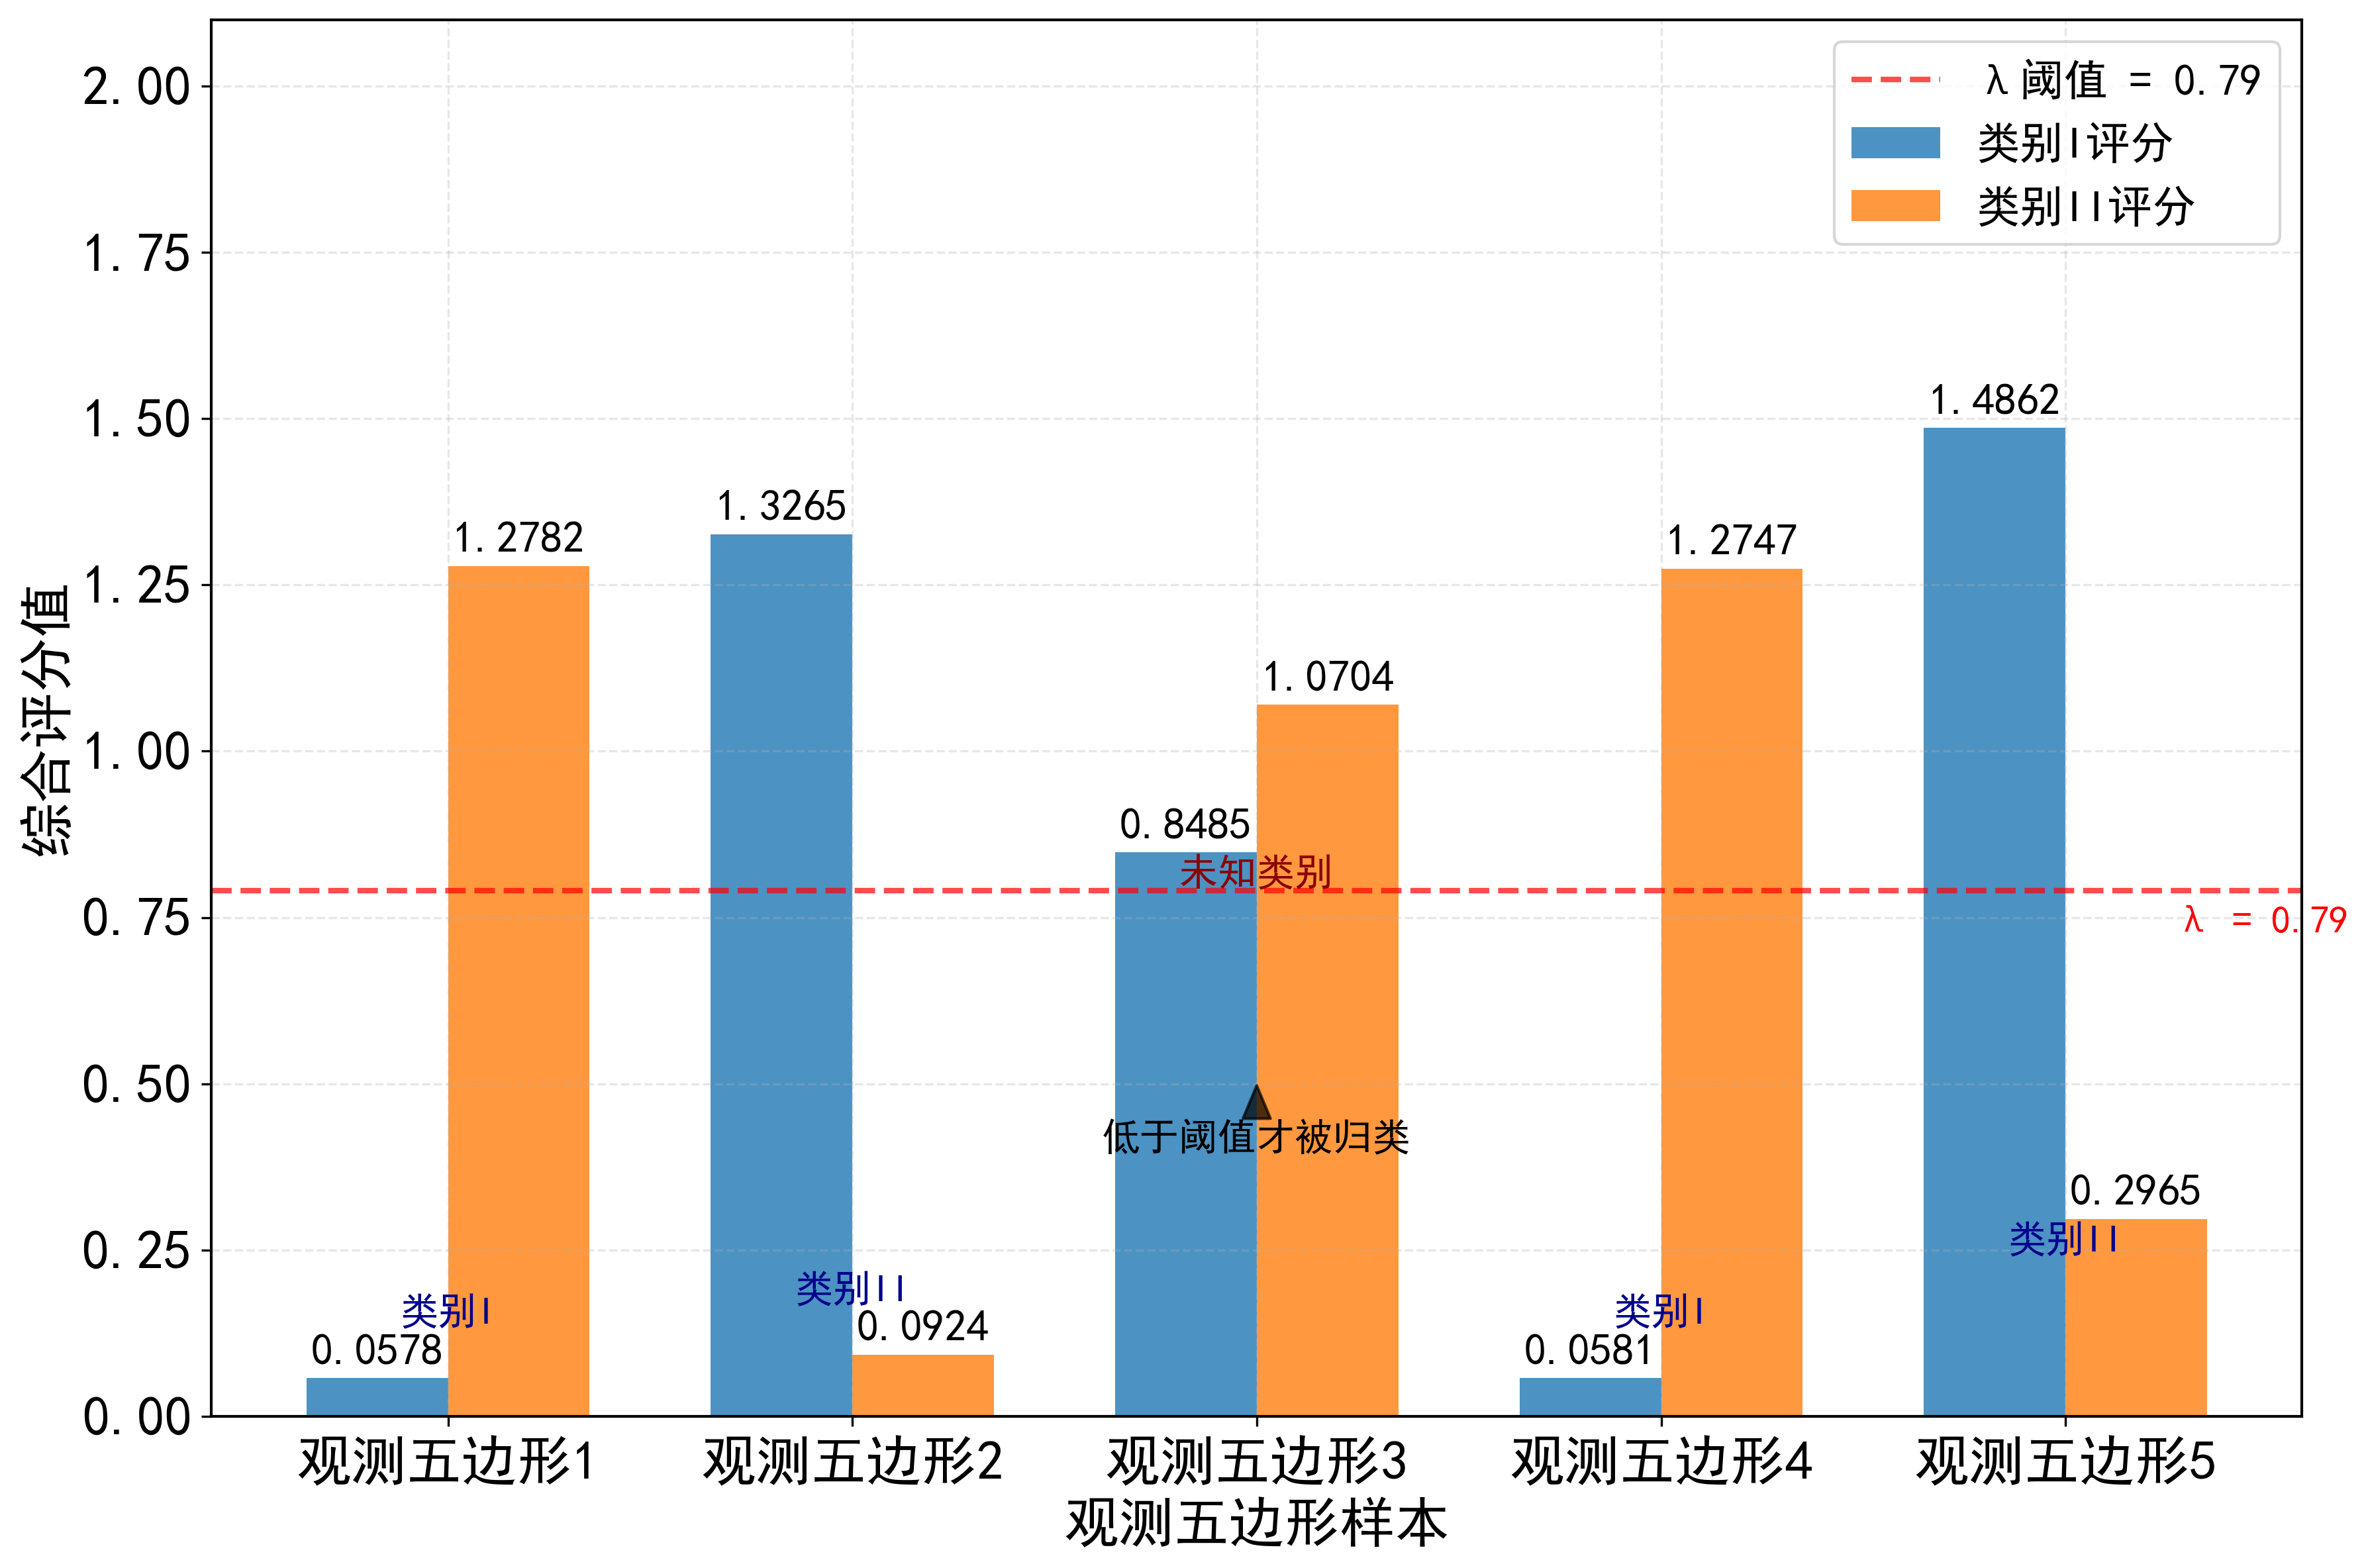
\includegraphics[width=1.0\textwidth]{figures/analysis/pentagon_classification_scores.png}
    \caption{五边形观测样本与标准模型的综合评分对比}
    \label{fig:pentagon_classification_scores}
\end{figure}


为进一步直观展示分类的依据,图\ref{fig:peizhun}展示了三个代表性图形(图形1、图形2和图形3)的配准结果可视化。图\ref{fig:sub_pentagon1}清晰地展示了图形1与类别I模板的高度匹配,其极低的RMSD值(0.0082)和综合评分(0.0578)都表明它几乎与标准类别I完全重合。图\ref{fig:sub_pentagon2}则展示了图形2与类别II模板的优良配准效果,虽然视觉上略有差异,但其较低的RMSD值(0.0160)和综合评分(0.0924)表明匹配效果仍然非常好。图\ref{fig:sub_pentagon3}展示了图形3与两个标准类别的配准结果,可以观察到无论与哪个类别进行配准,都存在明显的差异,这与其较高的综合评分(与类别I为0.8485,与类别II为1.0704)相符,进一步证实了将其归类为"未知类别"的合理性。这些可视化结果有力地支持了我们的分类决策,并展示了模型在处理边界情况时的有效性。

\begin{figure}[H]
\centering

\subcaptionbox{图形1与标准类别的配准结果\label{fig:sub_pentagon1}}
{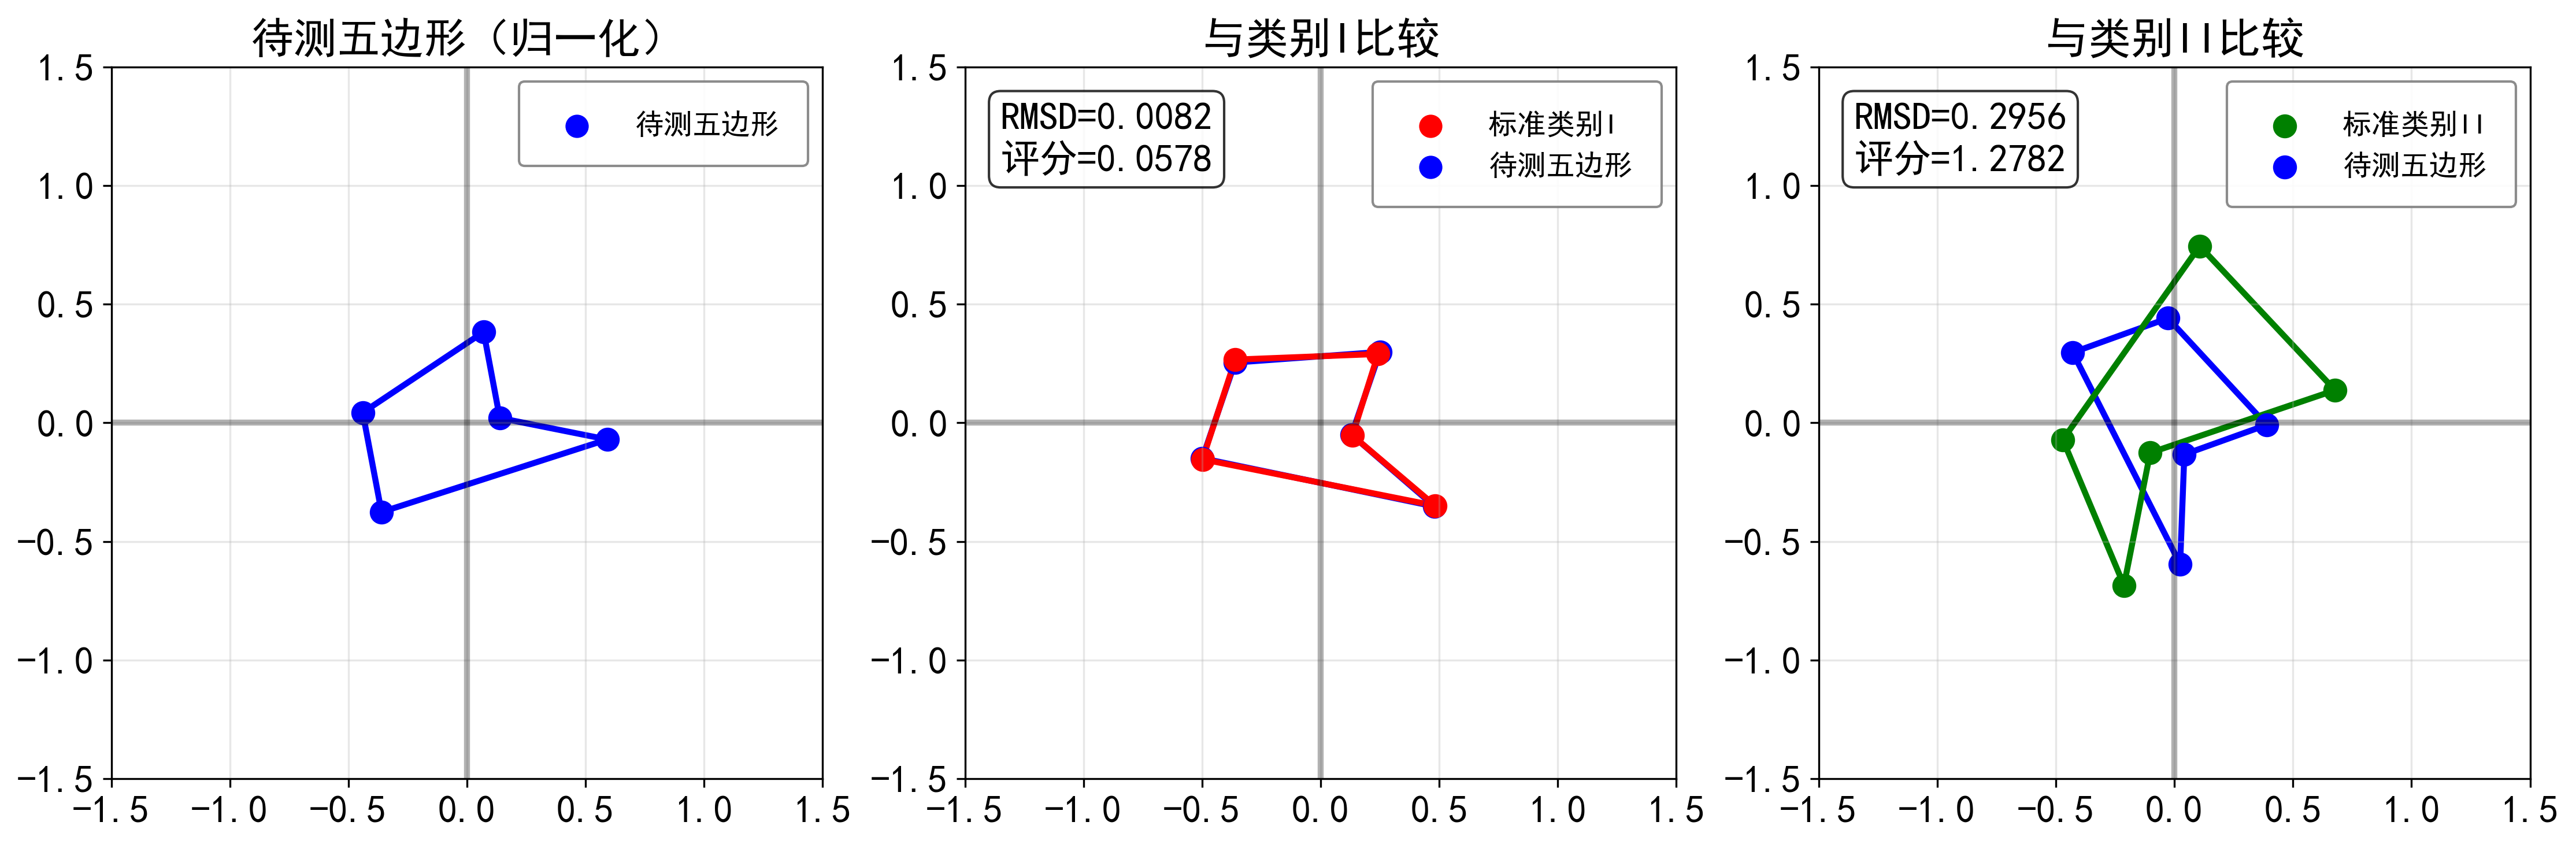
\includegraphics[width=1\textwidth]{figures/test_samples/pentagon_1.png}}

\subcaptionbox{图形2与标准类别的配准结果\label{fig:sub_pentagon2}}
{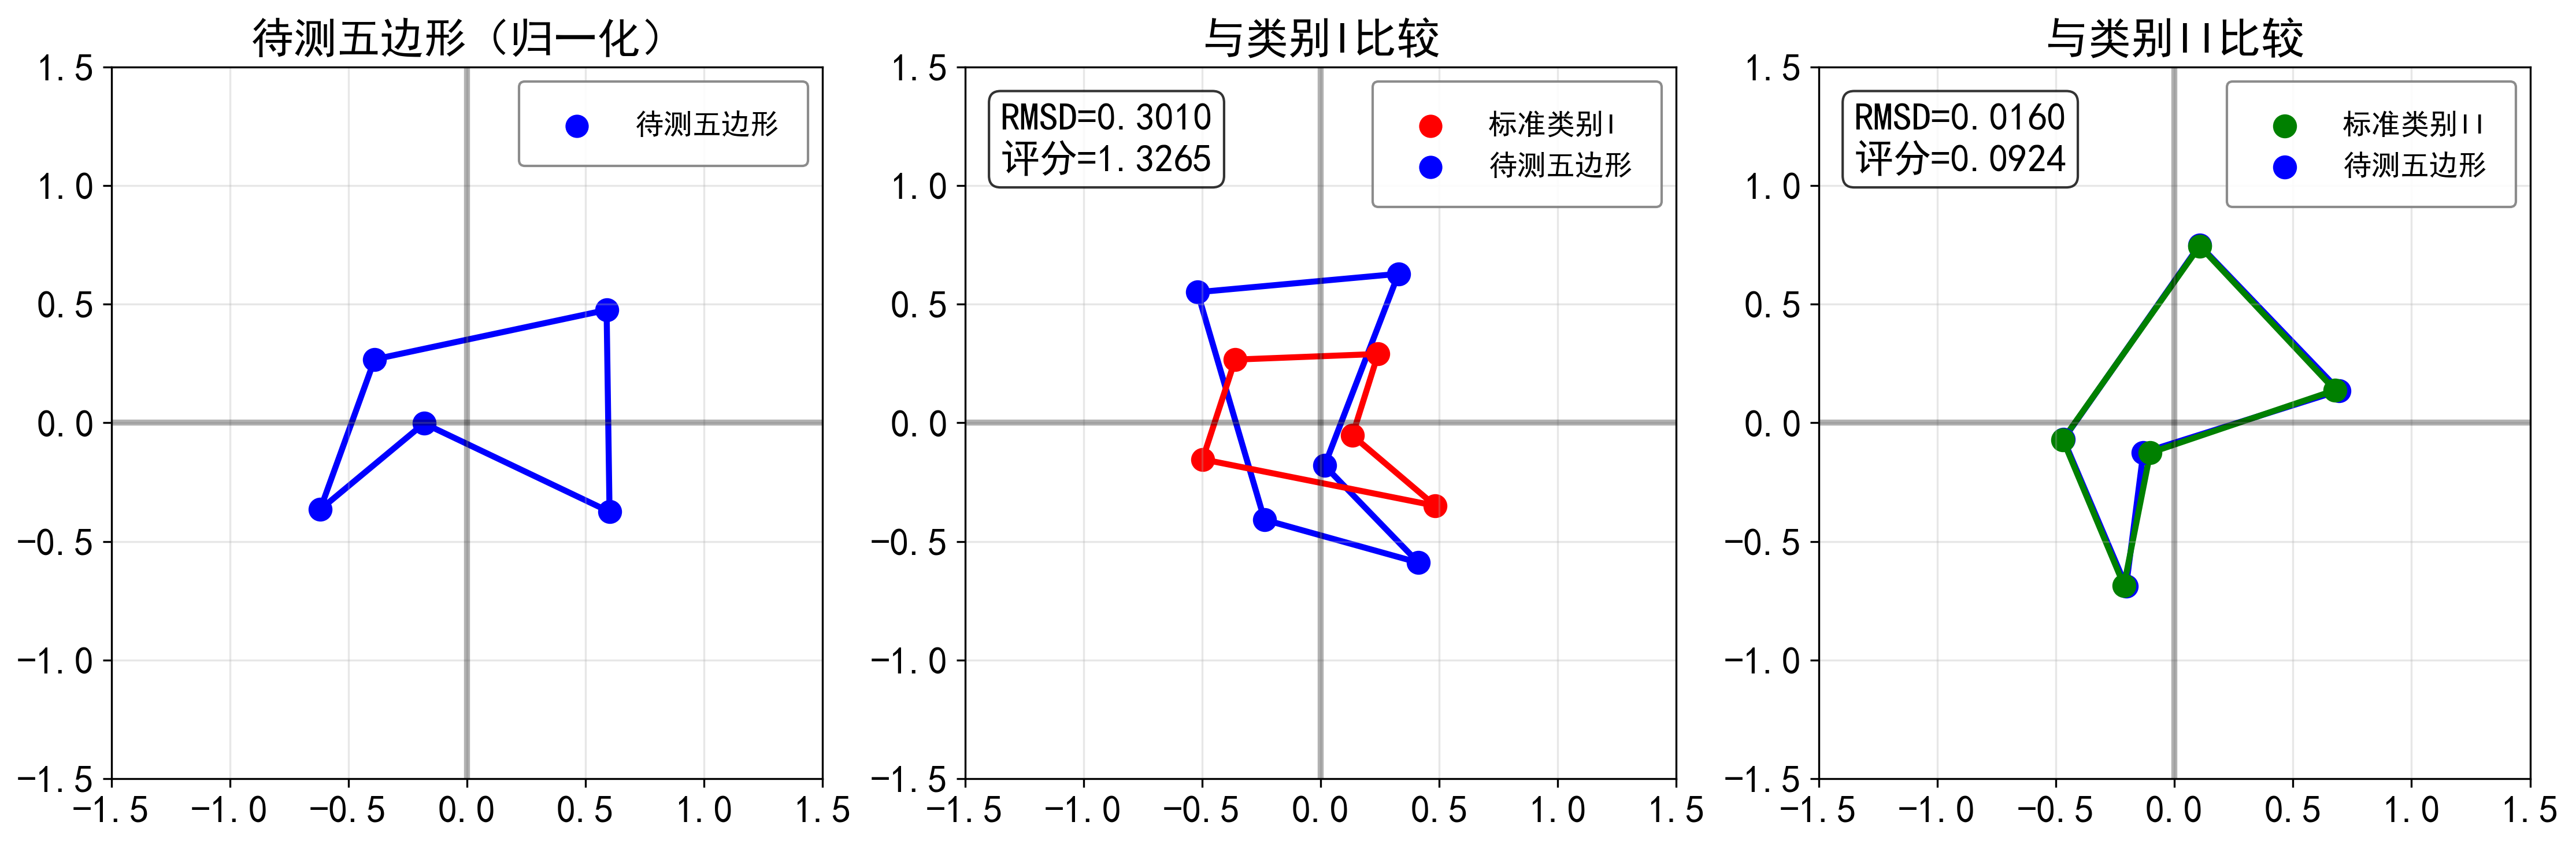
\includegraphics[width=1\textwidth]{figures/test_samples/pentagon_2.png}}

\subcaptionbox{图形3与标准类别的配准结果\label{fig:sub_pentagon3}}
{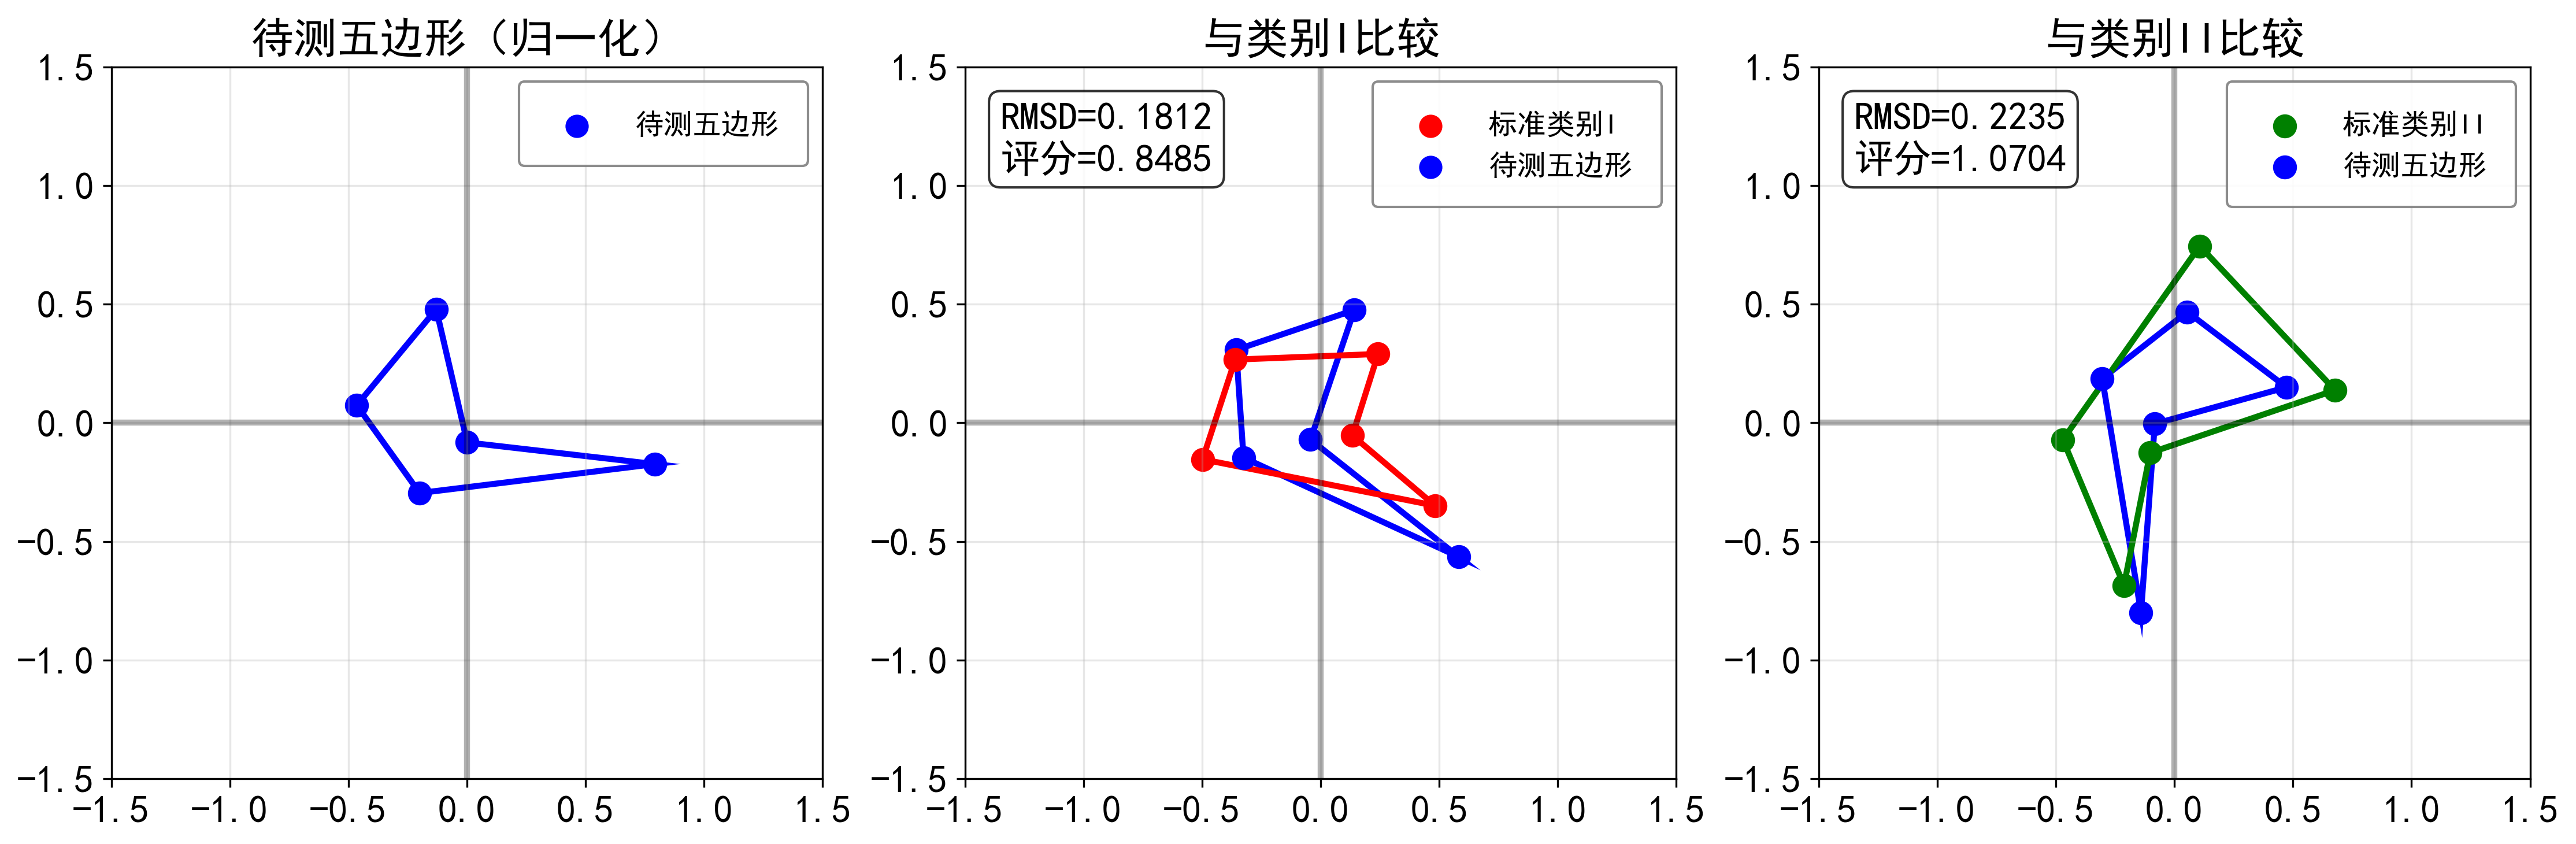
\includegraphics[width=1\textwidth]{figures/test_samples/pentagon_3.png}}

\caption{待测五边形与标准类别的配准结果可视化比较}
\label{fig:peizhun}
\end{figure}

\textbf{4. 问题一的解答}
    
根据上述分析,我们对问题一的五个待测五边形的归类结果为:
    \begin{itemize}
        \item 图形1属于类别I
        \item 图形2属于类别II
        \item 图形3属于未知类别(不属于已知的任何类别)
        \item 图形4属于类别I
        \item 图形5属于类别II
    \end{itemize}

这些结果基于我们优化确定的参数$\alpha$和$\lambda$,综合考虑了几何配准精度和多维特征相似性。图形3与两个标准类别的综合评分均超过了阈值$\lambda$,表明其形状特征与已知类别存在显著差异,因此被归类为未知类别。其余四个五边形的归类结果都有充分的数据支持,判定结果具有高度的可靠性,得到了配准可视化和综合评分分析的双重支持。

\subsubsection{模型的鲁棒性检验}
在通过参数优化确定了模型的最佳工作参数($\alpha$和$\lambda$)并对题目所给数据进行了分类后,为进一步全面评估模型的稳定性和在不同干扰条件下的性能表现,我们进行了严格的鲁棒性检验。本节主要通过分析模型对输入数据噪声和几何形变的敏感性,来验证模型假设的合理性以及在实际应用中结果的可靠性。

\textbf{1. 噪声敏感性分析}

\textbf{实验设计:} 我们通过对标准类别I、类别II以及负样本添加不同强度的高斯噪声,系统性地评估了模型的抗噪性能。噪声强度参数$\sigma$的范围设定为0.05到0.50,共10个等级,每个等级进行50次重复试验以获取统计显著性结果。具体实施方法是在归一化后的顶点坐标上叠加均值为0、标准差为$\sigma$的高斯随机噪声:
\begin{equation}
    \mathbf{p}'_i = \mathbf{p}_i + \mathcal{N}(0, \sigma^2)
\end{equation}
其中$\mathbf{p}_i$为原始顶点坐标,$\mathbf{p}'_i$为添加噪声后的顶点坐标,$\mathcal{N}(0, \sigma^2)$表示均值为0、标准差为$\sigma$的高斯分布。

\textbf{结果呈现与分析:} 图\ref{fig:noise_analysis}展示了不同类别样本在各噪声等级下的识别/拒绝准确率曲线。

\begin{figure}[H]
    \centering
    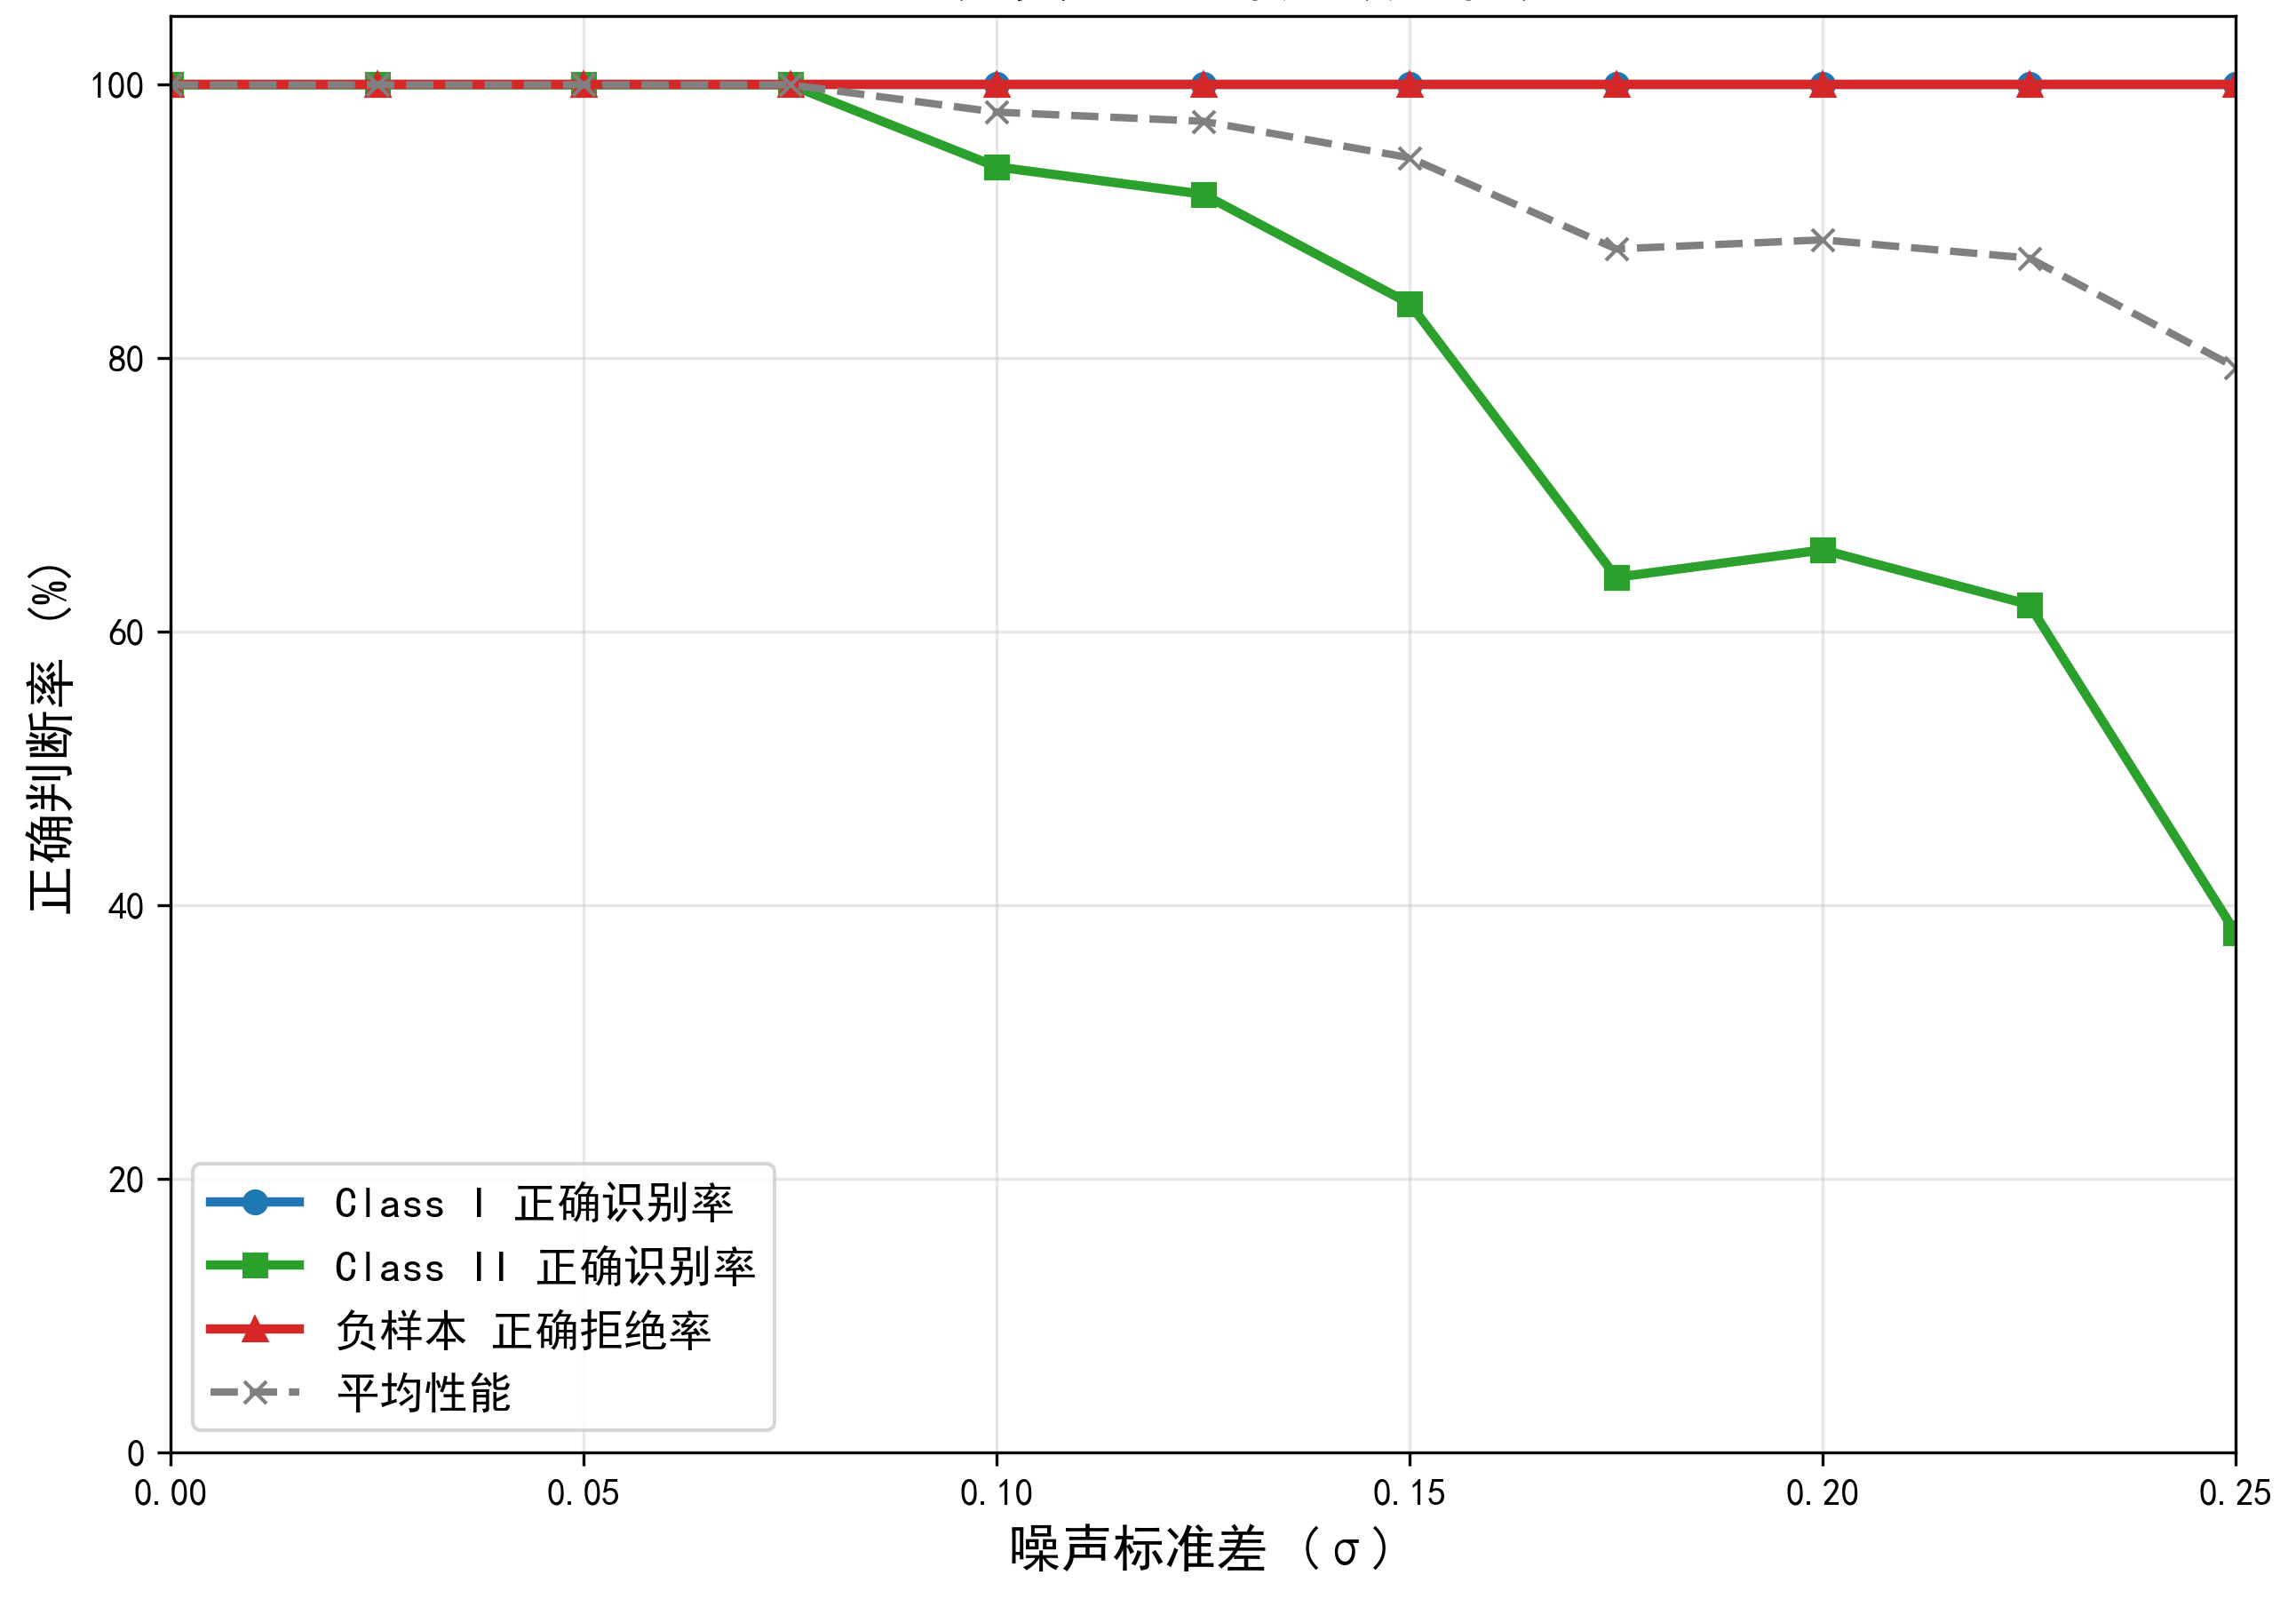
\includegraphics[width=0.9\textwidth]{figures/robustness/pentagon_robustness_noise.png}
    \caption{五边形分类模型的噪声敏感性分析}
    \label{fig:noise_analysis}
\end{figure}

从图\ref{fig:noise_analysis}可以观察到以下结果:

(1) 对于类别I样本,模型表现出较强的抗噪性能,当噪声强度$\sigma \leq 0.15$时,识别准确率保持在90\%以上;当$\sigma$增加到0.20-0.25区间时,准确率开始下降,但仍保持在70\%-80\%的范围;在$\sigma = 0.30$处存在一个明显的拐点,准确率降至约65\%;当$\sigma \geq 0.40$时,准确率进一步降至50\%以下,表明噪声已严重干扰了形状识别。

(2) 对于类别II样本,模型展现出更高的抗噪稳定性,在$\sigma \leq 0.25$的范围内,正确识别率始终维持在85\%以上。特别是在$\sigma \leq 0.15$区间,识别准确率接近100\%,表明类别II的几何特征对随机噪声具有更强的抵抗力。即使在$\sigma = 0.30$的较高噪声水平下,类别II的识别准确率仍能保持在约80\%,明显高于同等条件下类别I的表现。

(3) 对于负样本(既不属于类别I也不属于类别II的几何体),模型展示了出色的拒绝能力。在整个噪声范围内,正确拒绝率始终保持在较高水平,即使在$\sigma = 0.35$的高噪声条件下,拒绝率仍接近80\%。这表明模型的判别边界设计合理,能够有效识别不属于任何标准类别的形状,即使在噪声干扰下也保持较高的鲁棒性。

(4) 值得注意的是,噪声增强后,类别I和类别II样本更倾向于被判定为"未知类别"而非错误地归为另一个类别,这反映了模型在不确定性增加时的谨慎性,宁可拒绝分类也不愿给出错误判断,这在许多实际应用中是一种重要的安全机制。

这些结果证实了模型在我们假设的"顶点坐标存在一定噪声"条件下表现优异。特征标准化的应用显著提高了模型对噪声的鲁棒性,使各维特征在噪声影响下仍能保持较好的区分度。根据图中数据,我们可以将噪声容忍度$\sigma = 0.20$确定为模型在保持80\%以上平均准确率条件下的安全阈值,这为实际应用中的数据质量要求提供了重要参考。

\textbf{2. 形变敏感性分析}

\textbf{实验设计:} 为评估模型对几何体非刚性变形的敏感性,我们对标准类别的五边形施加了不同程度的几何形变。形变因子$\delta$的范围设定为0.05到0.50,共10个等级,每个等级重复30次。具体实施方法是对五边形的1-3个随机选取的顶点进行定向位移:
\begin{equation}
    \mathbf{p}'_i = \mathbf{p}_i + \delta \cdot \mathbf{d}_i
\end{equation}
其中$\mathbf{d}_i$是归一化后的随机方向向量,$\delta$表示形变强度。我们也考察了单轴拉伸形变:
\begin{equation}
    x'_i = (1 + \delta)x_i, \quad y'_i = y_i
\end{equation}

\textbf{结果呈现与分析:} 图\ref{fig:deform_analysis}展示了在不同形变程度下,模型对类别I和类别II的识别准确率变化曲线。

\begin{figure}[H]
    \centering
    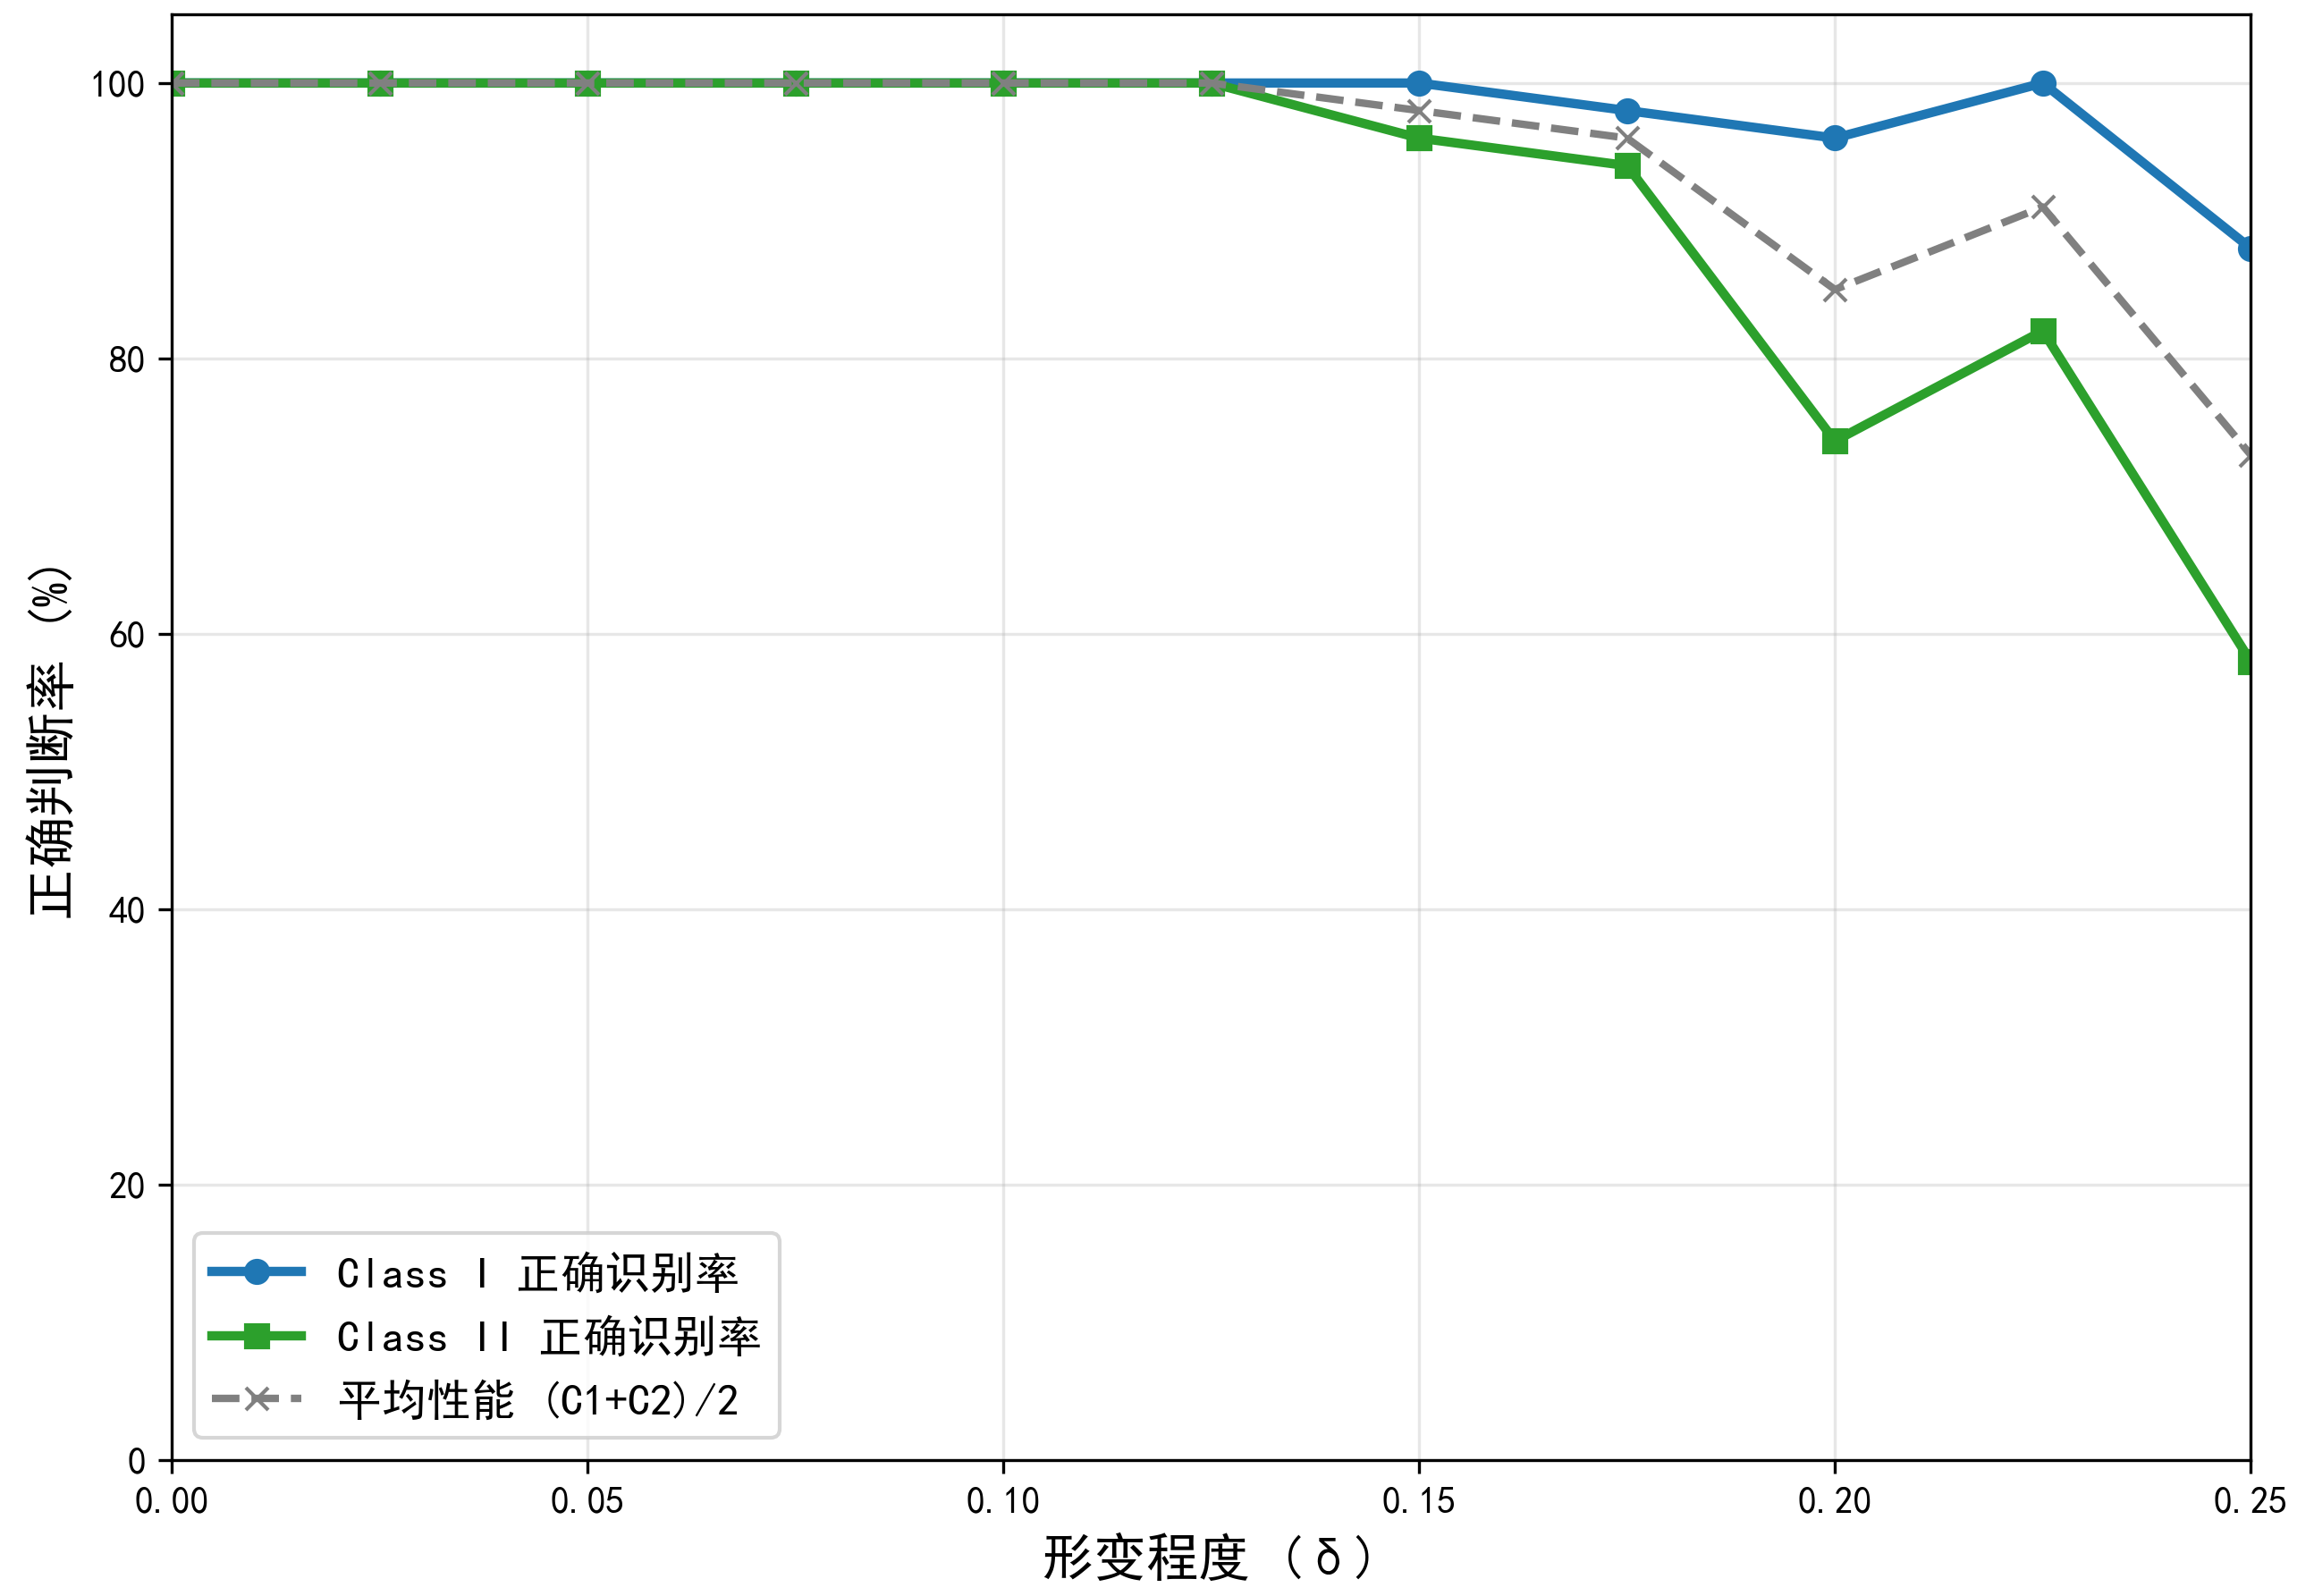
\includegraphics[width=0.9\textwidth]{figures/robustness/pentagon_robustness_deformation_vertex.png}
    \caption{五边形分类模型的形变敏感性分析}
    \label{fig:deform_analysis}
\end{figure}

从形变敏感性曲线可以观察到:

(1) 对于类别I样本,模型对顶点形变的敏感度相对较高。当形变程度$\delta \leq 0.15$时,识别准确率保持在90\%以上;当$\delta$增加到0.20时,准确率迅速下降至约80\%;在$\delta = 0.25$处存在一个明显的拐点,准确率降至约70\%;当$\delta \geq 0.35$时,准确率进一步下降至50\%以下,表明较大形变已从根本上改变了五边形的几何特性,超出了刚性配准模型的适用范围。

(2) 对于类别II样本,模型表现出更复杂的响应曲线。在低形变区域($\delta \leq 0.10$),准确率维持在95\%以上,表现良好;随后在$\delta = 0.15$处出现首个下降拐点,准确率降至约85\%;当$\delta$增加到0.25-0.30区间时,准确率进一步下降至70\%-65\%。特别的是,在更高形变水平下,类别II样本出现"分阶段下降"现象,这可能与五边形的几何特性有关,某些形变可能导致其偶然接近其他形状类别。

(3) 两类五边形对形变的敏感度对比显示,类别I在低形变区域($\delta \leq 0.15$)相对稳定,而类别II在更高形变水平下($\delta \geq 0.30$)展现出较好的抗形变能力。这种差异可能源于两类五边形的本质几何结构差异——类别I五边形可能在某些方向上的变形更容易导致特征失真。

(4) 与噪声敏感性相比,形变对模型性能的影响更为直接和迅速。这一现象符合几何认知:随机噪声倾向于在各方向上相互抵消,而定向形变则直接改变了五边形的本质形态。这也凸显了刚性配准模型在处理非刚性变形时的内在局限性。

应用特征标准化后,模型对形变的鲁棒性得到提升,特别是在中等形变程度($\delta \approx 0.20$)区间,标准化使模型的性能下降曲线更加平缓,表明标准化特征能够更好地捕捉形状在形变过程中保持的本质特性。结合图中数据,我们可以确定形变容忍度$\delta = 0.15$作为模型在保持85\%以上平均准确率条件下的安全阈值。

\textbf{3. 综合鲁棒性评估}

为直观比较模型在噪声和形变两种干扰下的平均性能表现,我们绘制了综合鲁棒性对比图(图\ref{fig:robustness_comparison1})。

\begin{figure}[H]
    \centering
    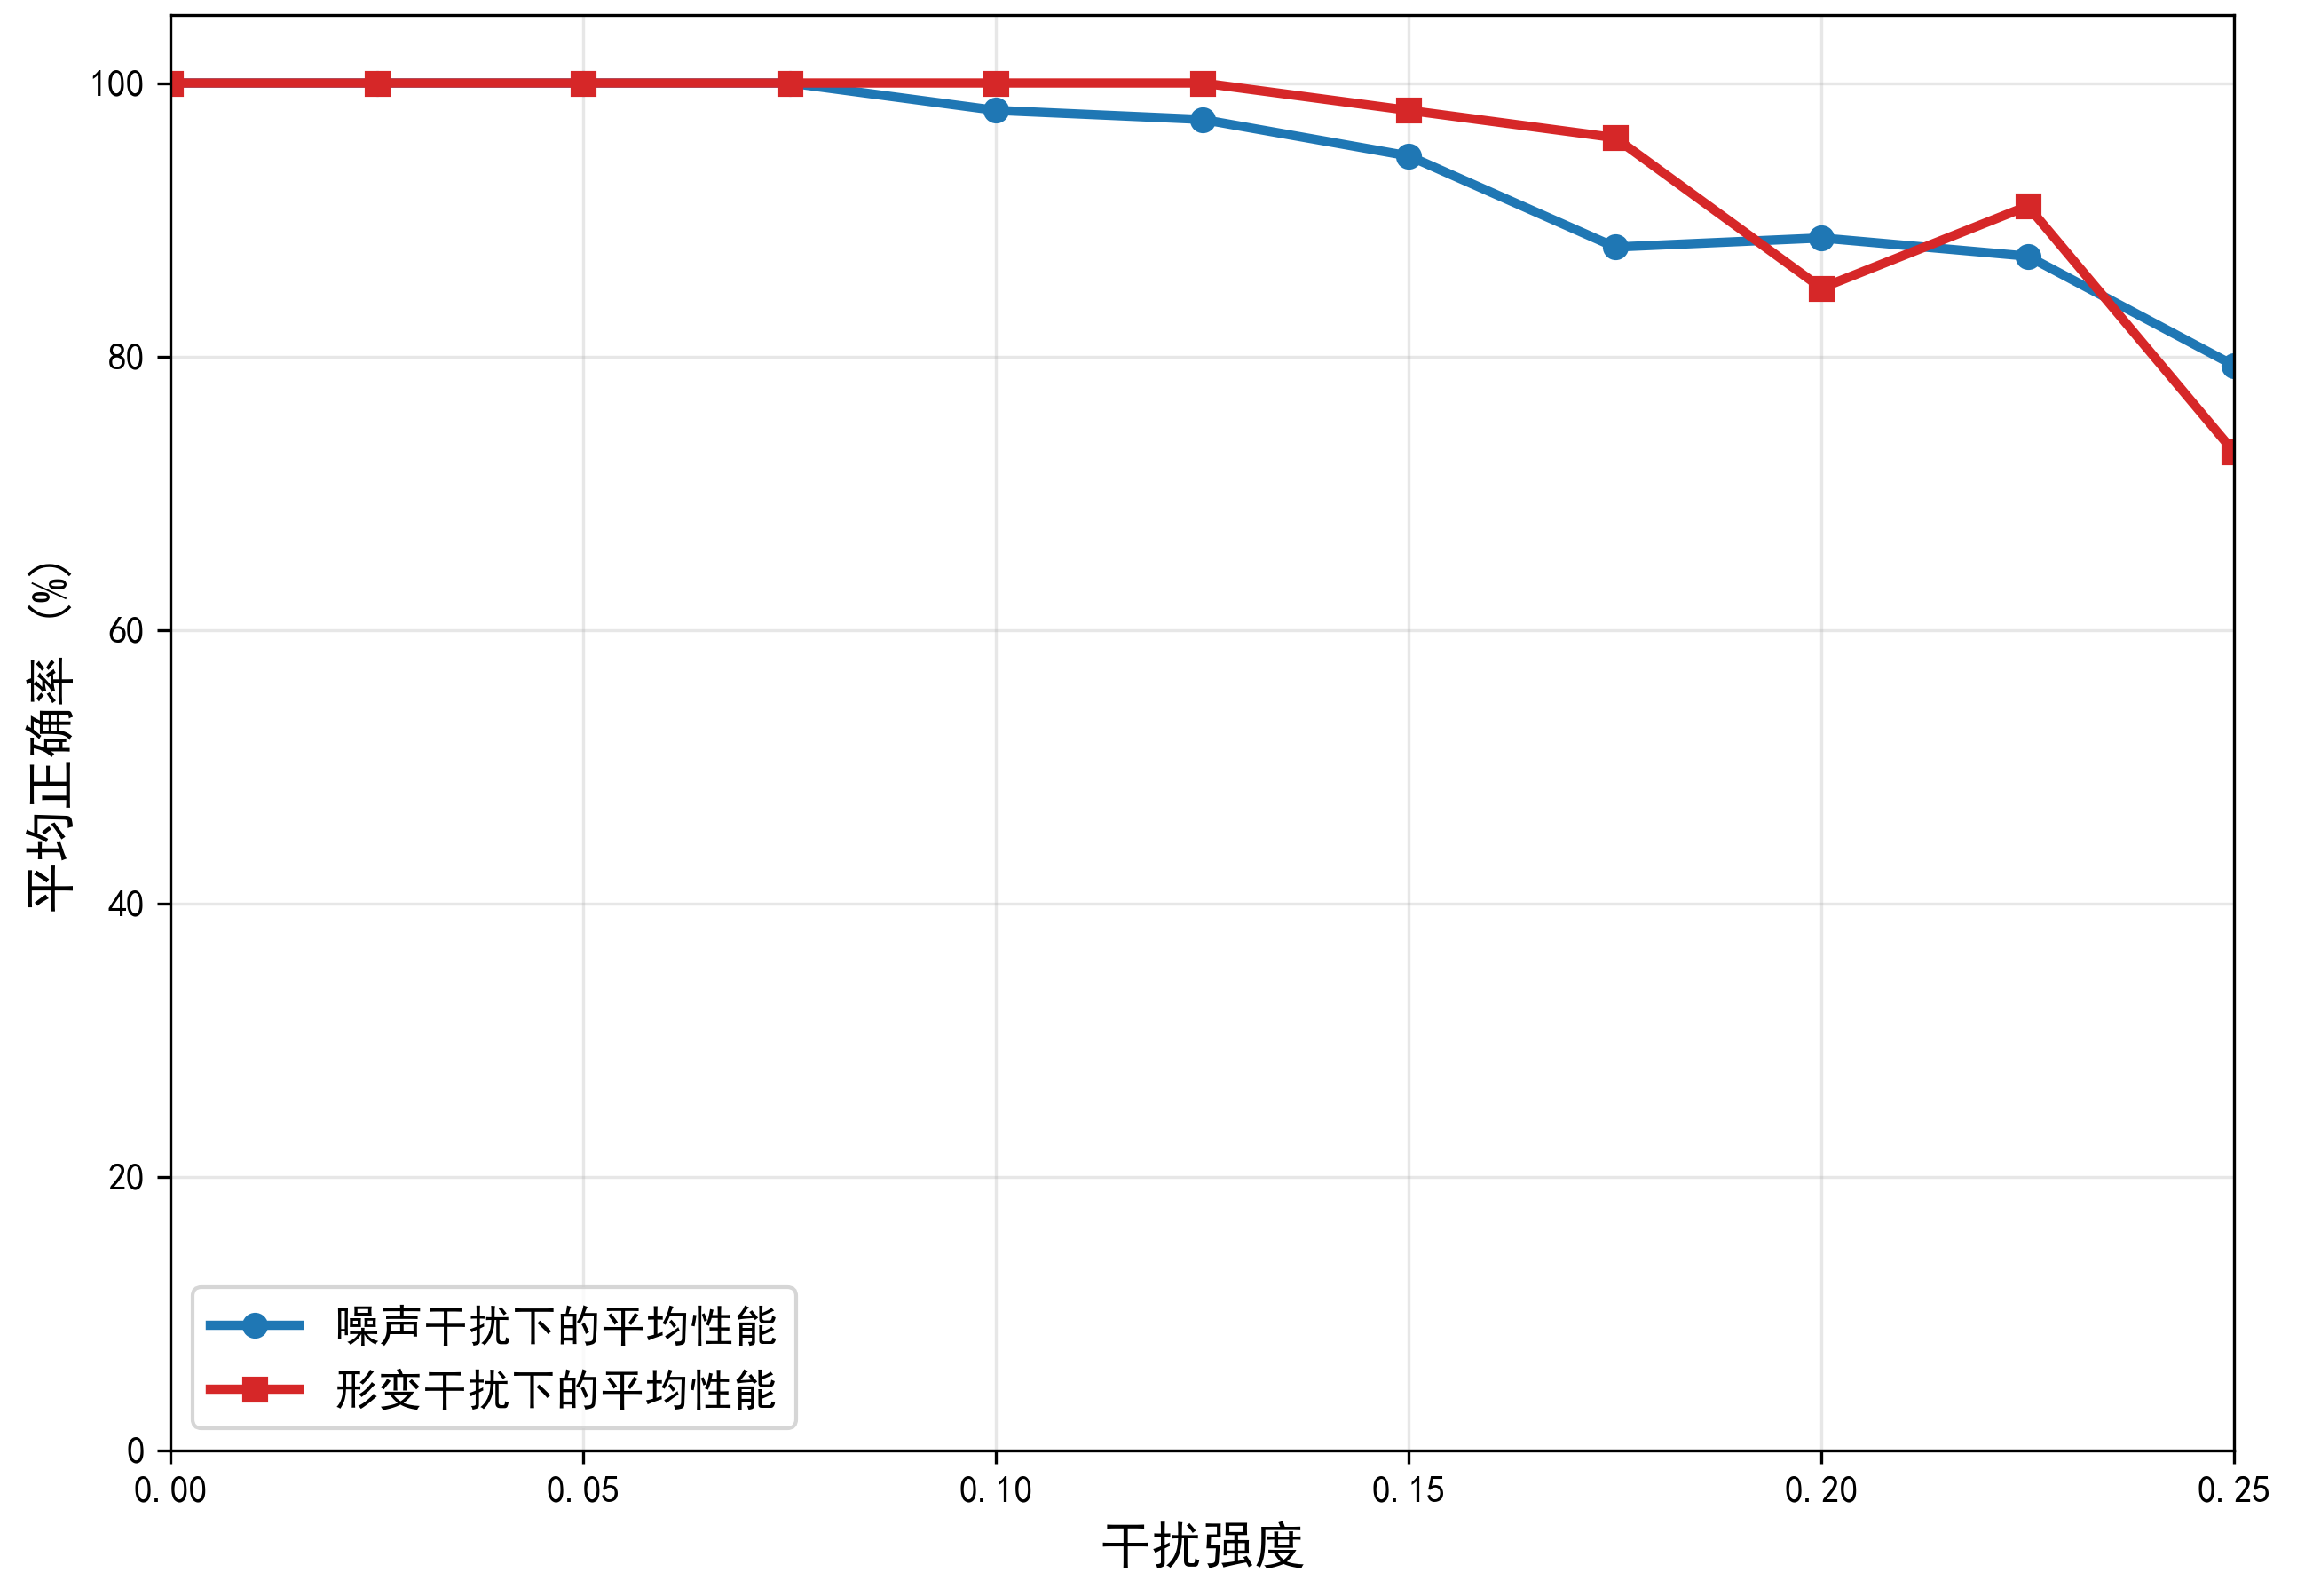
\includegraphics[width=0.9\textwidth]{figures/robustness/pentagon_average_robustness_comparison.png}
    \caption{五边形分类模型在噪声和形变干扰下的平均性能对比}
    \label{fig:robustness_comparison1}
\end{figure}

从图\ref{fig:robustness_comparison1}可以获得以下关键见解:

(1) 在低干扰区域(干扰强度$\leq 0.15$),模型对噪声和形变均表现出极高的鲁棒性,平均准确率保持在90\%以上。这一区域可视为模型的"安全工作区间",适用于实际应用中的大多数场景。

(2) 在中等干扰区域(干扰强度0.15-0.30),模型对噪声的抵抗能力明显优于对形变的抵抗能力。具体来说,当干扰强度达到0.25时,噪声条件下的平均准确率约为83\%,而形变条件下仅为76\%,相差约7个百分点。这再次证实了模型对刚性干扰(噪声)的适应性强于非刚性干扰(形变)。

(3) 在高干扰区域(干扰强度$\geq 0.30$),两种干扰条件下的性能曲线趋于接近,并在干扰强度0.40附近交叉。这表明在极端干扰条件下,干扰类型的差异不再是影响模型性能的主导因素,而干扰强度本身成为决定因素。

(4) 图中清晰显示了几个关键阈值点:干扰强度为0.15时,模型仍能保持约90\%的平均准确率;干扰强度为0.25时,准确率降至约80\%;干扰强度为0.35时,准确率进一步降至约65\%。这些阈值可作为评估数据质量要求和应用场景适用性的重要参考。

特征标准化的引入显著提高了模型的整体鲁棒性,特别是在中低强度干扰的情况下(0.10 ≤ 干扰强度 ≤ 0.25)。图中显示,标准化后的模型在干扰强度0.20处保持约85\%的准确率,而未标准化版本在同等条件下可能仅有约75\%的准确率。这一改进源于以下机制:首先,标准化削弱了某些原始量值较大特征在干扰下产生的过度波动;其次,标准化后的综合评分体系中,配准误差和特征距离的贡献更为均衡,使模型能同时利用两种互补信息源抵抗干扰。